\ifx\wholebook\relax \else

\documentclass{article}

\usepackage[nomarginpar
  %, margin=.5in
]{geometry}

\addtolength{\oddsidemargin}{-0.05in}
\addtolength{\evensidemargin}{-0.05in}
\addtolength{\textwidth}{0.1in}

\usepackage[cn]{../prelude}

\setcounter{page}{1}

\begin{document}

\title{无穷}

\author{刘新宇
\thanks{{\bfseries 刘新宇} \newline
  Email: liuxinyu95@gmail.com \newline}
  }

\maketitle
\fi

\markboth{无穷}{编程中的数学}

\ifx\wholebook\relax
\chapter{无穷}
\numberwithin{Exercise}{chapter}
\fi

\epigraph{我看到了,但我不相信。}{——1877年康托尔写给戴得金的信}

% "I see it, but I don't believe it." -- Richard Dedekind

\begin{wrapfigure}{R}{0.5\textwidth}
 \centering
 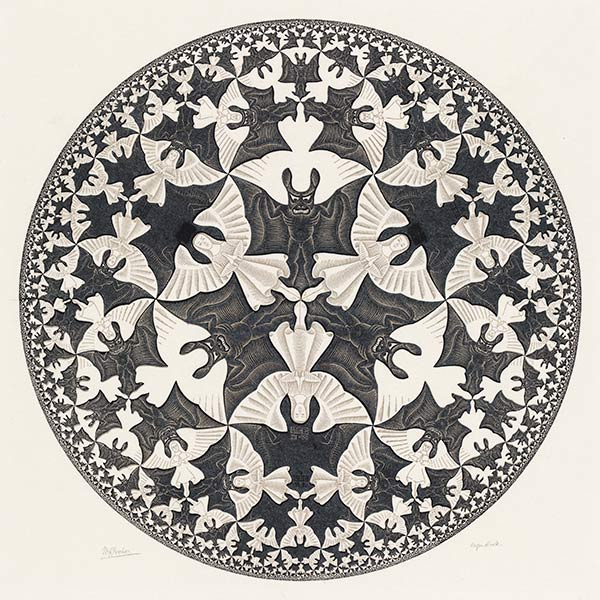
\includegraphics[scale=0.3]{img/circle-limit-IV-1960.eps}
 \captionsetup{labelformat=empty}
 \caption{埃舍尔《圆极限$\cdot$4》(又名天使与恶魔)1960}
 \label{fig:Circle-Limit-IV}
\end{wrapfigure}

不知在多久以前,我们的祖先仰望星空,面对浩瀚的星河,由衷地发出感叹,我们所在的世界究竟有多大?
作为智慧的生命,我们的思维超越自我,超越地球,超越宇宙,不断思考着无穷的概念。我们的祖先是从具体的事物中抽象出了数的概念。
例如狩猎得到的三头羊,采集得到三个果实,烧制了三个陶罐,进而得到抽象的数字三来代表任何三个东西。起初的数字大小有限,能够满足日常生活、狩猎、劳作的需要。
随着文明的发展,我们开始进行贸易活动,出于记账的要求,所需要的数字逐渐变大。人们发展出种种计数系统,来掌握更大的数字。
终于,我们提出问题:最大的数是什么?对于这个问题,人们分成了两种不同的态度。一种认为,这个问题没有意义,在古代,
掌握千百万这样的数已经足够在生活中使用了。我们无需了解生活中用不上的大数。例如可以认为世界上沙子的数目是无穷的。
在古希腊,一万曾被认为是一个十分巨大的数,人们称它为murias,最终变成了myriad一词,意为“无数”\cite{De-linfini-2018}。无独有偶,佛教中也用“恒河沙数”来表达大到无法计算的数。在大乘佛教经典《金刚经》中,佛陀说:“以七宝满尔所恒河沙数三千大世界,以用布施。”另一种则不这么想,阿基米德,这位古希腊伟大的数学家认为,即使是充满全宇宙的沙子数目,也可以用一个数代表。阿基米德在他的著作《数沙者》开篇中说:

“格朗王,有人认为沙子的数量是无穷的。我所说的沙子,并不单单地指叙拉古附近和西西里岛其余地方的沙子,还包括地球上所有角落能找到的沙子,无论那里有人还是无人居住。另一些人虽然承认沙子的数量并不是无穷大的,但他们认为,我们不可能写出一个足够大的数,使它在数量上超过地球上全部沙子所代表的数量。如果想象一个和地球体积同样大的沙体,而且要从地球上的大海和谷底算起,直到最高山峰的高度都填满沙子,这些人恐怕就更加肯定,世界上不可能有如此之大的数,可以用来表示堆积起这一巨大沙体所需要的沙子的数量。但是,我将向您证明,通过一系列几何证明——您之后也可以照着做——我命名了一些数字,写在我给宙克西珀的手稿中。其中一些数字不仅超过了以我刚刚描述过的方式填充地球所需要的沙子的数量,甚至超过了填充整个宇宙所需要的沙子数量。”

\begin{figure}[htbp]
%\begin{wrapfigure}{R}{0.4\textwidth}
 \centering
 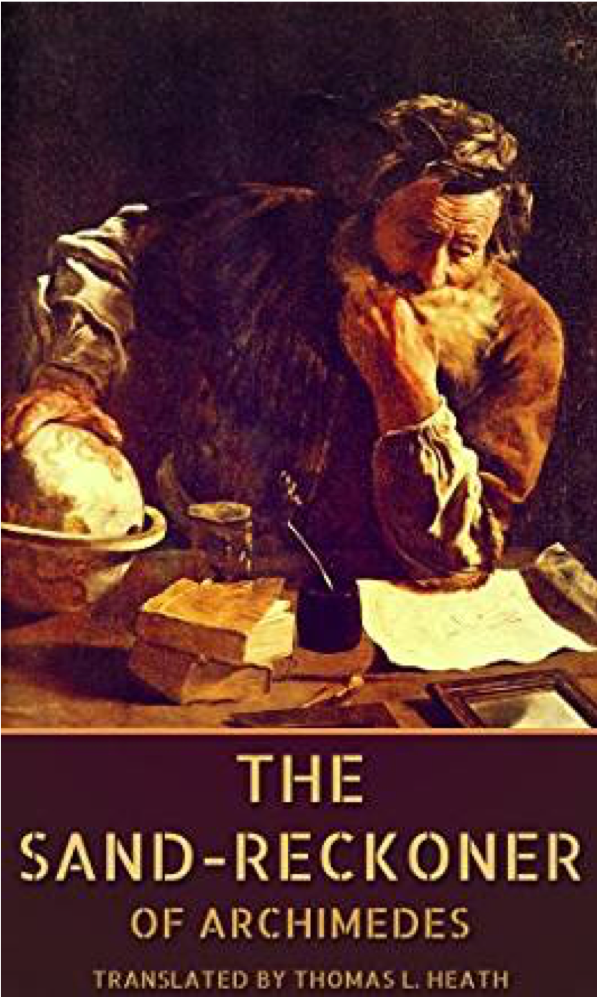
\includegraphics[scale=0.5]{img/Archimedes.eps}
 \captionsetup{labelformat=empty}
 \caption{《数沙者》,封面的阿基米德像是意大利画家多米尼克$\cdot$费蒂1620年创作的。}
 \label{fig:Archimedes}
%\end{wrapfigure}
\end{figure}

阿基米德认为填满宇宙“只”需要$10^{63}$粒沙子。这个宇宙的含义是指恒星天球,大约为两万倍地球的半径。今天我们知道可观测宇宙的尺寸大约为460亿光年,大约包含$3 \times 10^{74}$个原子\footnote{一说为$10^{80}$到$10^{87}$个基本粒子。}。在古希腊的时代,阿基米德的想法无疑是天才的,这几乎是无穷的具体化。我们从语言中,可以看到许多表达大数单位的词语。例如下表是汉语中的大单位,从“兆”以后,每增加一万倍,就有一个对应的单位。(\cite{Noguchi2007},第31页)

\begin{center}
% for Pinyin tones: \={a}, \'{a}, \v{}, \.{a}
\begin{tabular}{|l|r|l|r|}
\hline
京            & $10^{16}$ & 载            & $10^{44}$ \\
\hline
垓(g\={a}i)   & $10^{20}$ & 极            & $10^{48}$ \\
\hline
秭(z\v{i})    & $10^{24}$ & \textbf{恒河沙}  & $10^{52}$ \\
\hline
穰(r\'{a}ng)  & $10^{28}$ & 阿僧祗(zh\={i})  & $10^{56}$ \\
\hline
沟            & $10^{32}$ & 那由他        & $10^{60}$ \\
\hline
涧            & $10^{36}$ & 不可思议      & $10^{64}$ \\
\hline
正            & $10^{40}$ & 无量大数      & $10^{68}$ \\
\hline
\end{tabular}
\end{center}

可以看到,汉语中这些大单位词汇,有许多来自佛教。包括恒河沙,它表示1后面跟着52个0。英语中的大单位如下表。从一开始,每增加一千倍就有一个对应的单位。万进位和千进位的不同,也是文化上的一种差异。

\begin{center}
\begin{tabular}{|l|r|l|r|l|r|}
\hline
thousand & $10^{3}$ & quattuordecillion & $10^{45}$ & octovigintillion & $10^{87}$ \\
\hline
million & $10^{6}$ & quindecillion & $10^{48}$ & novemvigintillion & $10^{90}$ \\
\hline
billion & $10^{9}$ & sexdecillion & $10^{51}$ & trigintillion & $10^{93}$ \\
\hline
trillion  & $10^{12}$ & septdecillion & $10^{54}$ & untrigintillion & $10^{96}$ \\
\hline
quadrillion  & $10^{15}$ & octodecillion & $10^{57}$ & duotrigintillion & $10^{99}$ \\
\hline
quintillion  & $10^{18}$ & novemdecillion & $10^{60}$ & \textbf{googol} & $10^{100}$ \\
\hline
sexillion    & $10^{21}$ & vigintillion & $10^{63}$ & & \\
\hline
septillion   & $10^{24}$ & unvigintillion & $10^{66}$ & & \\
\hline
octillion    & $10^{27}$ & duovigintillion & $10^{69}$ & & \\
\hline
noniliion  & $10^{30}$ & trevigintillion & $10^{72}$ & & \\
\hline
decillion  & $10^{33}$ & quattuorvigintillion & $10^{75}$ & & \\
\hline
undecillion   & $10^{36}$ & quinvigintillion & $10^{78}$ & & \\
\hline
duodecillion  & $10^{39}$ & sexvigintillion & $10^{81}$ & & \\
\hline
tredecillion  & $10^{42}$ & seprvigintillion & $10^{84}$ & & \\
\hline
\end{tabular}
\end{center}

表中最后一个大单位古格尔(googol)是在1920年由9岁的米尔顿$\cdot$西洛塔(Milton Sirotta)想出的名字。这个数字是1后面跟着100个零。著名的互联网公司谷歌的名字就来自它\cite{Wikipedia-Googol}。

\section{无穷概念的提出}
\index{芝诺} \index{芝诺悖论}

超越一切具体大数的无穷是否存在不仅是一个数学问题,还是一个哲学问题。无穷大还直接导致另一个概念——无穷小。古代中国的哲学家庄子在《天下篇》中说:“一尺之棰,日取其半,万世不竭。”,古希腊的哲学家,埃利亚学派的芝诺(Zeno of Elea)提出了著名的四个悖论,它们都与无穷有关。

\begin{figure}[htbp]
%\begin{wrapfigure}{R}{0.3\textwidth}
 \centering
 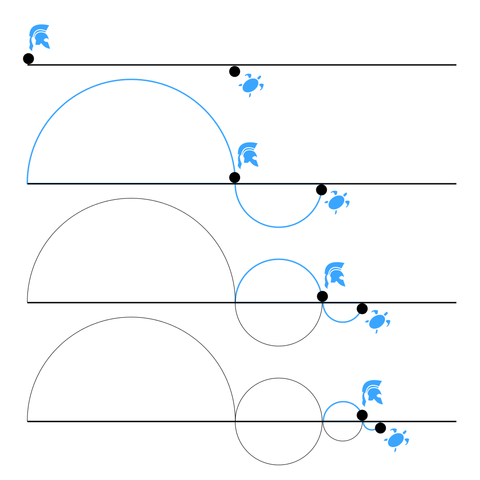
\includegraphics[scale=0.4]{img/Achilles-paradox.eps}
 %\captionsetup{labelformat=empty}
 \caption{阿基里斯与乌龟悖论}
 \label{fig:Achilles-paradox}
%\end{wrapfigure}
\end{figure}

第一个悖论最为人们所津津乐道。名叫阿基里斯与乌龟悖论。阿基里斯是荷马史诗《伊里亚特》中的英雄,以英勇著称。这个悖论说:如果让爬得很慢的乌龟在阿基里斯前面一段路程出发,那么阿基里斯将永远追不上乌龟。这是因为,阿基里斯为了赶上乌龟,必须先到达乌龟的出发点$A$,但当阿基里斯到达$A$点时,乌龟已经在这段时间前进到了$B$点。但当阿基里斯到达$B$点时,乌龟又已经到了前面的$C$点……以此类推,两者间的距离虽然越来越近,但阿基里斯永远落在乌龟的后面而追不上乌龟。如图\ref{fig:Achilles-paradox}所示。但是这与我们生活中的常识是不相符的。这个悖论的推理是如此让人信服,以至于千百年来吸引了无数学者的研究。刘易斯$\cdot$卡罗尔(Lewis Carrol)、侯世达(Douglas Hofstadter)甚至拿乌龟和阿基里斯作为文学作品中的主人公。

第二个悖论叫作“二分悖论”。这个悖论的主人公是希腊神话中善于疾走的女猎手阿塔兰塔。如果阿塔兰塔想从$A$到$B$,那么她必须先走到$1/2$的位置。同样在此之前,她必须要到达$1/4$的位置。而为了到达这一位置,她必须先到达$1/8$的位置……以此类推。由于这样的中点有无限多个,阿塔兰塔永远也也无法到达目的。芝诺的这个悖论实际上说明了运动根本无法发生。

\begin{figure}[htbp]
%\begin{wrapfigure}{R}{0.3\textwidth}
 \centering
 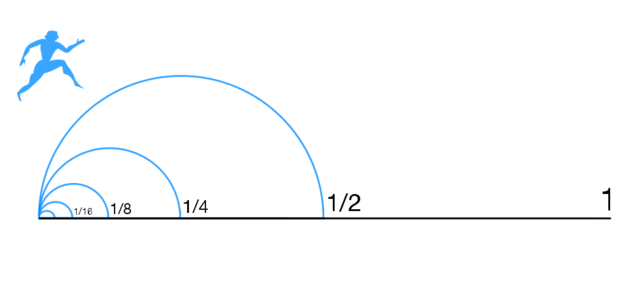
\includegraphics[scale=0.4]{img/Dichotomy-paradox.eps}
 %\captionsetup{labelformat=empty}
 \caption{二分悖论}
 \label{fig:Dichotomy-paradox}
%\end{wrapfigure}
\end{figure}

第三个悖论叫作“飞矢不动悖论”,它从另一个角度描述无穷导致运动无法发生。芝诺指出,任何物体待在相同的位置都不叫运动,可是飞行的箭矢在任一时刻不也是待在一个地方么?这样说来,自然飞失也是不动的。如果说前两个悖论是由于分割空间导致的,则这个悖论是由对时间的分割导致的。

\begin{figure}[htbp]
%\begin{wrapfigure}{R}{0.3\textwidth}
 \centering
 %\subcaptionbox{飞失不动悖论}[0.3\linewidth]{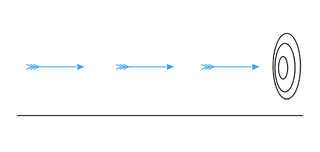
\includegraphics[scale=0.4]{img/Arrow-paradox.eps}}
 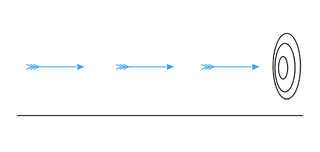
\includegraphics[scale=0.4]{img/Arrow-paradox.eps}
 \caption{飞失不动悖论}
 \label{fig:Arrow-paradox}
\end{figure}

第四个悖论叫作“运动场悖论”。这一悖论主要针对时间原子论的观点,即认为存在最小的不可分割的时间单位。如图\ref{fig:Moving-rows-paradox}所示,运动场中有3列人。最初他们都首尾对齐。在最小的时间单元内,A列不动,B向右移一个单位,而$\Gamma$向左移动一个单位。容易得知,相对B而言,$\Gamma$其实移动了两个单位。这就意味着,应该存在这一让$\Gamma$相对于B移动一个单位的时间。而这一时间应该是最小单位时间的一半。但如果存在不可分割的“时间原子”,那么这两个时间就是相同的,即最小时间和它的一半相等。

\begin{figure}[htbp]
 \centering
 %\subcaptionbox{运动场悖论}[0.7\linewidth]{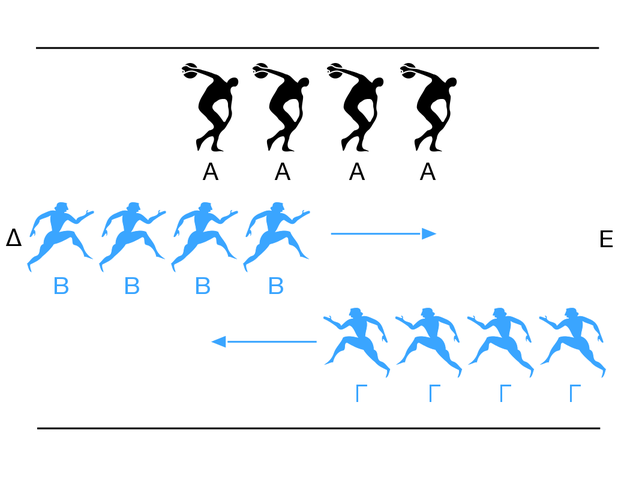
\includegraphics[scale=0.3]{img/Moving-rows-paradox.eps}}
 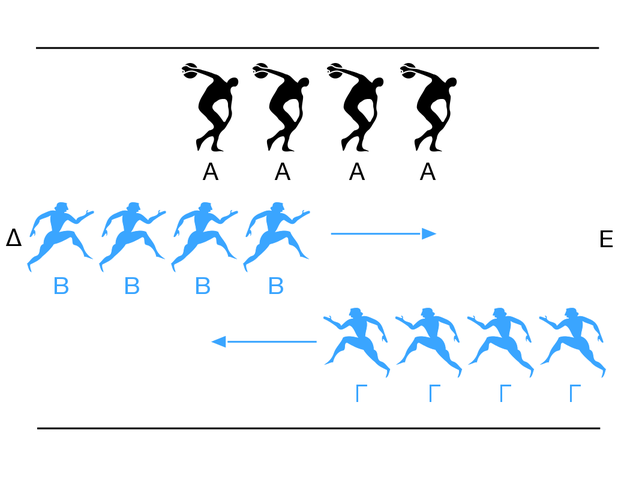
\includegraphics[scale=0.3]{img/Moving-rows-paradox.eps}
 \caption{运动场悖论}
 %\captionsetup{labelformat=empty}
 \label{fig:Moving-rows-paradox}
%\end{wrapfigure}
\end{figure}

芝诺悖论并不复杂,稍加琢磨就能理解。但是导出的结果却出人意料。根据生活中的常识,运动和时间是如此真实,阿基里斯不可能赶不上乌龟。可是驳倒这些悖论却并不容易,从亚里士多德到罗素,从阿基米德到赫尔曼$\cdot$外尔,都对芝诺悖论提出了各种不同的解法\cite{Wikipedia-Zeno}。

芝诺(约公元前490年——公元前425年),古希腊哲学家,生于意大利半岛南部的埃利亚。所以我们常称其为埃利亚的芝诺。关于他的生平,缺少可靠的文字记载。据传,他早年是一个自学成才的乡村孩子,一生经历坎坷,最终遭到一位暴君的陷害而被拘捕、拷打、直至被处死\cite{HanXueTao16}。

芝诺是继毕达哥拉斯学派之后在意大利新出现的一个哲学学派——埃利亚学派的代表人物之一,这一学派的领袖是芝诺的老师巴门尼德。巴门尼德认为整个世界是个不变的整体,即“不变的一”,运动、变化与多样性都只是幻象。

芝诺以其悖论闻名。他一生曾巧妙地构想出40多个悖论,在流传下来的悖论中以关于运动的四个“无限微妙、无限深邃”的悖论最为著名。他提出这些悖论很可能是为他老师的哲学观点辩护。

\begin{figure}[htbp]
%\begin{wrapfigure}{L}{0.3\textwidth}
 \centering
 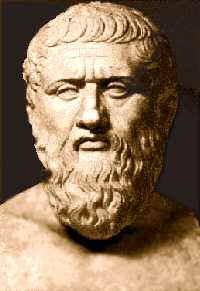
\includegraphics[scale=0.5]{img/Zeno.eps}
 \captionsetup{labelformat=empty}
 \caption{芝诺,约490BC - 425BC}
 \label{fig:Zeno-of-Elea}
%\end{wrapfigure}
\end{figure}

芝诺悖论在当时曾给古希腊人造成深深的困惑。而芝诺悖论所涉及的对时间、空间、无限、连续、运动的看法,也都在极长的历史岁月中困扰着后来的哲学家和数学家。如何了解和认识无穷,如何使用无穷成为了摆在古希腊人面前必须解决的问题。

\subsection{无穷的哲学}
\index{潜无穷} \index{实无穷}
亚里士多德对芝诺悖论进行了深入的思考(我们今天对芝诺悖论的了解,其实是来自亚里士多德的著作《物理学》),并做出一项对后世数学发展具有深远影响的工作。他把无穷的概念区分为实无穷和潜无穷。所谓潜无穷或潜无限,是指无限在永远延伸着,是一种变化的、不断产生出来概念。它永远在构造中,永远完成不了,是潜在的,而不是实在的。自然数就是一种潜无穷,对于任何一个自然数,我们都可以找到它的后继,也就是一个更大的自然数。欧几里得几何中的直线也是一种潜无穷,我们可以按需延伸直线\footnote{欧几里得避免使用“无限延伸”这样的说法,而代之以按需任意延伸。这在古希腊是常见的一种处理。}。所谓实无穷是指把无限的整体本身作为一个实在的单位,是已经构造出来的东西。也就是把无限对象看作可完成的过程或无穷整体。

在做了这种区分后,亚里士多德承认存在潜无穷,但是拒绝承认实无穷的概念。他对实无穷的排斥深刻而长远地影响了日后数学的发展\cite{HanXueTao16}。亚里士多德代表了当时古希腊的哲学观点,关于潜无穷和实无穷的概念区分以及争论一直影响至今。尽管对无穷的概念仍然心存疑虑,古希腊的数学家们借助潜无穷的思想取得了令人赞叹的成就。其中之一就是欧几里得证明了存在无穷多的素数。这一证明被人们认为是历史上最优美的证明之一。

\begin{theorem}
《几何原本》第九卷,命题20。预先给定任意多的素数,则有比它们更多的素数\cite{Elements}。
\end{theorem}

欧几里得在叙述这个命题时,小心谨慎地避免使用无穷这样的说法,通观《几何原本》一书这样的例子还有很多。欧几里得在证明这个命题时,使用了著名的反证法。我们用现代的语言来描述这一证明。

\begin{proof}
假设只存在有限多个素数,$p_1, p_2, ..., p_n$。我们构造一个新数:
\[
p_1 p_2 ... p_n + 1
\]
也就是把这$n$个素数乘起来再加一。这个数要么是素数,要么不是素数。

\begin{itemize}
\item 如果它是素数,明显这个数不等于$p_1$到$p_n$中的任何一个,这就在有限多个素数中又增加了一个新的素数;
\item 如果这个数不是素数,那么它就存在一个素因子$p$。但是由于$p_1$到$p_n$中的任何一个都不能整除我们构造的这个数,所以素数$p$与任何$p_1$到$p_n$中的数都不同,是一个新的素数。
\end{itemize}
所以在任何情况下,我们都可以获得一个新的素数。这与有限个素数的假设矛盾,因此存在无穷多的素数。
\end{proof}

欧几里得用反正法得到了一种“存在性证明”,他证明了存在无穷多的素数,但却没有给出怎样得到这些素数。这在我们今天看来,是很自然的一种处理。然而在十九世纪末二十世纪初却引发了关于数学根本性的争论,我们将在下一章详细讲述这一内容。

\begin{figure}[htbp]
%\begin{wrapfigure}{L}{0.3\textwidth}
 \centering
 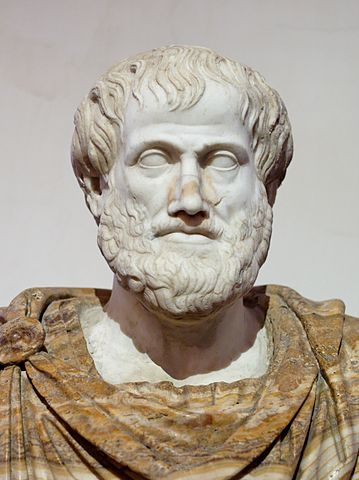
\includegraphics[scale=1]{img/Aristotle.eps}
 \captionsetup{labelformat=empty}
 \caption{亚里士多德,384BC - 322BC}
 \label{fig:Aristotle}
%\end{wrapfigure}
\end{figure}

\index{亚里士多德}
亚里士多德是世界古代史上最伟大的哲学家、科学家和教育家之一,古希腊哲学的集大成者。他是柏拉图的学生,亚历山大大帝的老师。公元前384年,亚里士多德出生于希腊北部城市斯塔基拉(Stageira)。后人对他早年的生活所知甚少。17岁时,他赴雅典在柏拉图学园就读达20年,直到柏拉图去世后方才离开。这一时期的学习和生活对他一生产生了决定性的影响。苏格拉底是柏拉图的老师,亚里士多德又受教于柏拉图。在雅典的柏拉图学园中,亚里士多德表现得很出色,柏拉图称他是“学园之灵”。但亚里士多德可不是个只崇拜权威,在学术上唯唯诺诺而没有自己的想法的人。他努力地收集各种图书资料,勤奋钻研,甚至为自己建立了一个图书室。

公元前347年,柏拉图去世。两年后,亚里士多德离开了雅典——亚里士多德或许是带着失望的心情离开的,因为他并没有成为柏拉图思想的继承者。此后,他开始游历各地。公元前343年,亚里士多德被马其顿的国王腓力浦二世召唤回故乡,受国王的聘请,担任起当时年仅13岁的亚历山大大帝的老师。亚里士多德也运用了自己的影响力,对亚历山大大帝的思想形成起了重要的作用。正是在亚里士多德的影响下,亚历山大大帝始终对科学事业非常关心,对知识十分尊重。

公元前335年腓力浦去世,亚里士多德又回到雅典,并在那里建立了自己的学校。学园的名字叫做吕克昂(Lyceum)。在此期间,亚里士多德边讲课,边撰写了多部哲学著作。亚里士多德讲课时有一个习惯,边讲边漫步于走廊和花园,正是因为如此,学园的哲学被称为“逍遥派”或者是“漫步的哲学”。亚里士多德在这一期间也有很多著作,主要是关于自然学和物理方面的自然科学和哲学,而使用的语言也要比柏拉图的《对话录》晦涩许多。他的作品很多都是以讲课的笔记为基础,有些甚至是他学生的课堂笔记。因此有人将亚里士多德看作是西方的第一个教科书作者。

亚历山大去世后,雅典人开始奋起反对马其顿的统治。由于和亚历山大的关系,雅典人攻击亚里士多德,并判他为不敬神罪,当年苏格拉底就是因不敬神罪而被判处死刑的。但亚里士多德最终逃出了雅典。

公元前322年,亚里士多德因身染重病离开人世,终年六十三岁。

亚里士多德重视研究现实世界,他的精神财富正在于他的实证研究方法,这成为了现代科学的基本原则。此外,现在大学里面的院系划分方式,及其所反应的知识整理方式,也直接沿承自亚里士多德所提出的分类法。

\subsection{穷竭法与微积分}
\index{穷竭法}
与欧几里得的小心谨慎不同,古希腊的另一些数学家采用了较为实用的态度对待无穷,创造并发展了一种称为“穷竭法”的有力工具,取得了惊人的成就。

穷竭法由古希腊智人学派的代表人物安提丰(Antiphon,约前480——前410)首创。为了解决古希腊三大作图难题之一的圆化方问题\footnote{亦称为化圆为方问题,另外两个著名的难题是三分角问题和倍立方问题。任给一个圆,古希腊人希望找到只用尺规,能够作出同样面积的正方形。这个问题困扰了无数的数学家,直到19世纪后利用伽罗瓦的理论,才一举将它们题解决。三大难题被证明都是尺规不可解的。在英文中化圆为方square the circle被形容不可能做到的事情。},他提出用圆内接多边形逼近圆面积的方法来化圆为方。安提丰从一个圆内接正方形开始,不断将边数加倍得到正八边形、十六边形……不断重复这一过程,随着圆面积的逐渐“穷竭”,将得到一个边长越来越微小的圆内接正多边形。安提丰认为最终这一正多边形将与圆重合,这就是穷竭法的思想。后来古希腊伟大的数学家欧多克索斯对穷竭法进行了改进和严格化,使其成为解决面积、体积问题的一种有力的几何方法。为了理解这一方法,我们先要介绍著名的欧多克索斯——阿基米德公理,有时简称为阿基米德公理。

\index{阿基米德公理}
\begin{axiom}
\textbf{阿基米德公理(Axiom of Archimedes)}对于任意两个量$a$与$b$来说,总有自然数$n$使得$a \leq nb$。
\end{axiom}

阿基米德公理非常基本。在第二章中,我们介绍了欧几里得最大公约数算法,但是我们没有探讨这一算法是否能够结束。利用阿基米德公里就可以给出欧几里得算法一定能够结束的证明。利用这一基本原理,欧多克索斯指出:“给定两个不相等的量,如果从较大的量减去比它大一半的量,再从所余的量减去比这个余量大一半的量,重复这一过程,必有某个余量小于给定的较小的量。”这就是穷竭法背后的逻辑。

利用穷竭法,欧多克索斯证明了棱锥体积是同底同高棱柱体积的1/3,圆锥体积是同底同高圆柱体积的1/3。这些成果都记录在欧几里得的《几何原本》卷12中\cite{HanXueTao16}。

古希腊将穷竭法发展到最高成就的当属阿基米德,他取得了惊人的成就,计算出了圆周率$\pi$,证明圆面积公式,球体、锥体的表面积和体积公式,甚至找到了计算抛物线下面积的方法。被称为古希腊的数学之神。

%\begin{figure}[htbp]
\begin{wrapfigure}{R}{0.4\textwidth}
 \centering
 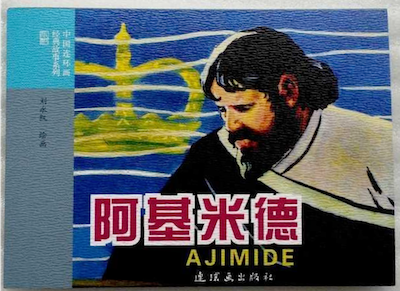
\includegraphics[scale=0.6]{img/Archimedes-book.eps}
 \captionsetup{labelformat=empty}
 \caption{小儿书《阿基米德》的封面}
 \label{fig:Archimedes-book}
\end{wrapfigure}
%\end{figure}

\index{阿基米德}
阿基米德(前287年——前212年),生于西西里岛的叙拉古王国。早年曾经在古希腊的学术中心亚历山大城跟随欧几里得学习。阿基米德后来回到了叙拉古,他的许多学术成果都是通过和亚历山大城的学者之间的往来信件保存下来的。虽然有关阿基米德的生平没有详细的记载,但是关于他的各种故事却广为流传、脍炙人口。

最著名的故事就是国王的王冠。叙拉古国王不知道他的王冠是否是纯金的,大臣们也一筹莫展,于是去请教阿基米德。阿基米德一直解不开这个难题,他废寝忘食,直到有一天洗澡的时候,看着浴缸里的水溢出来,突然得到了灵感。他从浴缸里一跃而出,光着身子跑到大街上,边跑边喊“尤里卡!尤里卡!”,这句希腊语Eureka的意思是“我找到了!”。阿基米德利用浮力和比重,最终发现王冠掺了假。他的这一发现就是每一个中学生都要学习的“阿基米德定律”。尤里卡后来被人们用来形容找到灵感的那一刹那。

阿基米德发现球的体积是其外接圆柱体积的2/3。他觉得这一关系无比的美妙,因此决定死后在墓碑上刻一个内接圆柱的球体。
% Sphere: 4/3 pi r^3, Cylinder: pi r^2 * 2r = 2 pi r^3
% ==> S : C = 4/3 / 2 = 2/3

公元前214年,第二次布诺战争爆发了。面对敌人的围城,传说阿基米德设计了巨大的抛物面镜,把阳光汇聚到帆上烧毁了敌人的战船。阿基米德还设计了巨大的机械武器,可以瞬间击毁罗马战船。后来罗马军队攻陷了叙拉古城,一个罗马士兵冲进阿基米德家里。阿基米德正专注地在沙地上画着几何图形进行思考,他说出了那句著名的画:“你挡住了我的阳光。”感到被冒犯的罗马士兵挥刀杀死了面前的这个老人。古希腊最伟大的数学家就此停止了思考。

我们现在来看一下,阿基米德是如何利用穷竭法计算圆周率的。

如图\ref{fig:pi-exhaustion}所示,阿基米德在直径为1的圆内做一个内接多边形,同时在圆外做一个外切多边形。我们先看内接多边形的一条边和其上的圆弧,根据两点之间直线最短的几何公理,圆弧之长大于内接多边形的一条边长,故而圆的周长大于内接多边形的周长。同样可以得知,圆的周长小于外切多边形的周长。由于直径为1的圆,其周长恰好就是圆周率。这样我们就可以得到关系式:

\[
  C_i < \pi < C_o
\]

\begin{figure}[htbp]
%\begin{wrapfigure}{R}{0.4\textwidth}
 \centering
 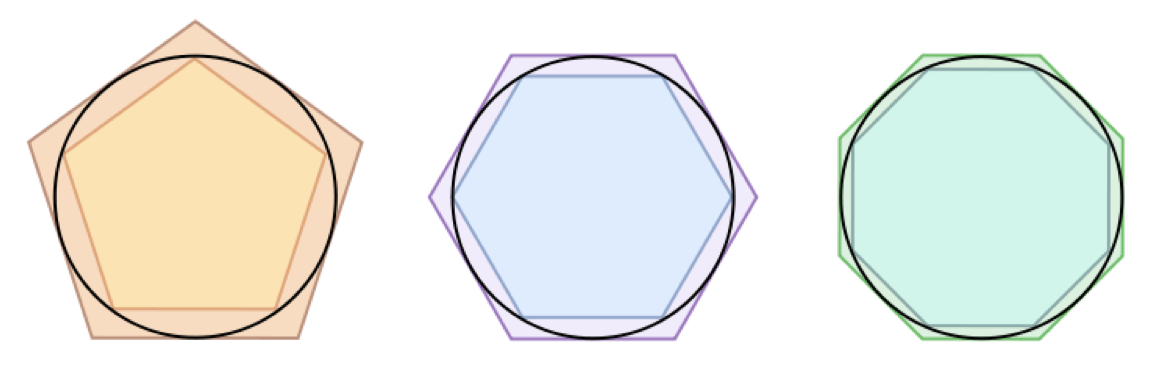
\includegraphics[scale=0.5]{img/pi-exhaustion.eps}
 %\captionsetup{labelformat=empty}
 \caption{用穷竭法计算圆周率}
 \label{fig:pi-exhaustion}
%\end{wrapfigure}
\end{figure}

其中$C_i$、$C_o$分别为内接多边形和外切多边形的周长。不断加大边数,就可以越来越精确地获得$\pi$的范围。阿基米德将边数加到96,得出圆周率在3.1408和3.1429之间。400年后,古希腊天文学家托勒密用穷竭法将精度提高到3.1416。这一记录直到南北朝时,才由我国的数学家祖冲之打破。

穷竭法的缺点是,它仍然是基于古希腊几何的一种方法,使用起来非常复杂。这部分是由于古希腊人不接受无理数,于是把几何量和“数”的概念隔离开。另一方面,古希腊整体上试图避免使用无穷大和无穷小的概念。

另一位使用穷竭法的大师是天文学家托勒密。他首次为天体运行建立了模型,地球位于宇宙的中心,月球,太阳,和其他行星则在嵌套于一起的球面上运行,最外层则是恒星天球。

亚历山大时代之后,古希腊文明的数学成果遭受了巨大的打击。罗马人征服后,迪奥多西(Theodosius)废除了异教,并于392年下令拆毁古希腊人的神庙。成千上万的希腊图书被罗马人焚毁。在公元前47年,罗马人纵火焚烧亚历山大港口内的船只,火势蔓延烧毁了藏书最丰富的古代图书馆。保存大量希腊著作的塞拉皮斯神庙也被摧毁,写在羊皮上的著作被刮掉而改写宗教著作。

对希腊文明的最后打击是公元640年新崛起的阿拉伯帝国对埃及的征服。残剩的图书被焚毁殆尽。征服者奥马尔说:“这些书的内容或许我们也有,那么我们不必读它;这些书里或许有反对我们的内容,那我们不准读它。”因此亚历山大城的浴室里接连有6个月用羊皮纸来烧水\cite{M-Kline-2007}。

每次读到此处的历史,不仅让人痛心疾首,唏嘘不已。焚书的悲剧在南美洲,在秦帝国,自古及今不断上演。埃及被占领后,一些学者迁居到东罗马帝国的首都君士坦丁堡。阿拉伯帝国后来也把一部分古希腊的数学著作翻译成阿拉伯文。巴格达的智慧宫成为了当时世界学术的中心。中世纪后,欧洲的学者又逐渐把这些阿拉伯文的著作再次译成拉丁文。伴随着文艺复兴,也是数学和哲学的复兴。接过阿基米德和穷竭法的接力棒的是德国天文学家约翰内斯$\cdot$开普勒。托勒密的宇宙模型无法解释行星反向运动的现象,于是不得不引入了本轮、匀轮、偏心圆和匀速点的概念。通过分析行星的观测数据,哥白尼提出了日心说,从托勒密模型需要的78个圆简化到了34个圆。但仍然和观测有一些偏差。开普勒潜心分析德国天文学家第谷的数据8年,终于破解了行星运动的规律,这就是我们今天熟知的开普勒三大行星运动定律。按照开普勒定律,行星的运行轨迹并不是圆,而是一个椭圆,太阳在椭圆的一个焦点上。行星在单位时间内扫过的面积相同,因而在椭圆上有时速度快(例如在近日点附近),有时速度慢(例如在远日点附近)。分析这样复杂的数学模型需要新的工具,古希腊的穷竭法太过复杂笨重。开普勒于是进行了简化,他甚至还用自己简化的方法计算出了葡萄酒桶的容积。

接下来迈出重要一步的是笛卡尔和费马。通过解析几何,人们终于将数和几何结合了起来,并且在莱布尼茨和牛顿的手中发展出了微积分。微积分中的一个绕不开的概念是无限小量。并且在积分中必然要涉及无限多个量的累加。值得一题的是1665年,对微积分的发展做出重要贡献的学者约翰$\cdot$沃利斯首次引入了现代的无穷符号$\infty$。

尽管微积分的基础尚有很多争论,这一代表西方现代精神的风帆在18世纪乘风破浪。这是一个英雄辈出的时代,伯努利家族、欧拉、拉格朗日奔放地使用着微积分和无穷级数,解决了一个又一个以前无法想象的难题,在天文学,力学、流体力学上开拓进取。

\section{潜无穷与编程}
对微积分基础的严密化直接导致了人们对实无穷的思考与激烈争论。在此之前,我们先来看一下在编程中,无穷是如何被体现的。计算机使用的是有限的资源,历史上,整数在机器内部表示为二进制形式。因为只用有限的二进制位,所以能表示的整数范围也是有限的。$m$位二进制最大可以表示$2^m-1$的整数,它的二进制形式为11...1,即$m$个1。例如16位整数的最大值是$2^{16}-1 = 65535$。由于这个原因,如果多个元素集合的基数用整数表示,则元素的数目也是有限的。在传统的编程中,常使用数组来容纳多个元素,为了节省内存通常要求事先确定数组大小的上限,例如下面的C语言程序定义了一个容量为10个元素的整数数组:

\begin{verbatim}
int a[10];
\end{verbatim}

这里涉及两个概念,一个是序数,一个是基数。简单来说,序数就是我们在数数时赋予对象的一个标签。而基数是一个集合中元素的个数。我们稍后会给出它们的一般定义。早期的编程中,基数和序数都是有限的。这显然无法直接表达无穷的概念。在计算机科学发展的初期,这是完全可以理解的。那时的设备非常昂贵。人们根本不会想到使用无穷来直接解决具体的问题。然而随着时代的发展,成本逐渐降低,人们不再满足在解决问题之前,先预测出所需集合的大小。于是在一些编程环境中,开始支持动态增长的数组。人们称之为容器或者向量,可以随时按照需要向其中增加元素。现实中,即使是动态容器,其中的元素个数仍然是有限的,不能超过表示的上限。为此人们又发展出了链表结构。如本书第一章中介绍的那样,每个元素用一个节点代表,一个接一个链接起来,最后一个元素指向一个特殊的空节点表示结尾。这样我们无须知道整条链表的基数,却能从表头开始,逐一前进到表中任何位置。只要存储空间允许,链表可以任意长。这样就创造了表达潜无穷的可能。

可是链表和潜无穷终究还差了一步。我们认为自然数是无限延伸着的潜无穷,如果用链表表示自然数,不管链表有多长,例如$n$,我们必须把0到$n$这些数都逐一填入其中。但这只表示了序列0, 1, ..., $n$,而不是自然数序列0, 1, ..., $n$, ...

\index{惰性求值}
为此,人们提出了惰性求值的概念。所谓惰性求值,就是并不立即计算一个变量的值,而是把计算推迟到需要这个值的时候。具体到自然数的例子,根据第一章介绍的皮亚诺公理,任给一个自然数$n$,都存在它的后继$n+1$。而第一个自然数是0。这样自然数就可以表示为:

\[
N = iterate(n \mapsto n + 1, 0)
\]

其中$iterate$的定义为:

\[
iterate(f, x) = x : iterate(f, f(x))
\]

我们来看一下自然数产生的头几步,简单起见,我们命名$succ(n) = n \mapsto n +1$

\[
\begin{array}{rcll}
iterate(succ, 0) & = & 0 : iterate(succ, succ(0)) & iterate\text{的定义}\\
                 & = & 0 : iterate(succ, 1) & succ(0) = 0 + 1 = 1 \\
                 & = & 0 : 1 : iterate(succ, succ(1)) & \\
                 & = & 0 : 1 : iterate(succ, 2) & \\
                 & = & 0 : 1 : 2 : iterate(succ, 3) & \\
                 & = & ... & \\
\end{array}
\]

如果没有惰性求值,上述过程就会一直计算下去,永不终止。这是无法用来解决实际问题的。为此我们必须把链表的链接操作实现为惰性的,其中一种方法就是利用第二章介绍的$\lambda$表达式:

\[
x : xs = cons(x, () \mapsto xs)
\]

这种表达式$() \mapsto exp$通常叫作$delay(exp)$,它产生一个不带有参数函数,对这个函数求值得到结果$exp$。

\begin{figure}[htbp]
%\begin{wrapfigure}{R}{0.4\textwidth}
 \centering
 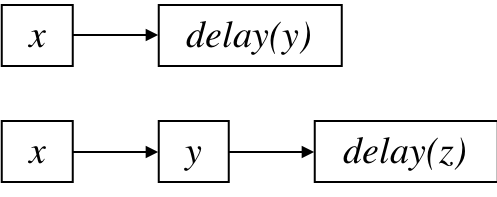
\includegraphics[scale=0.5]{img/stream-cons.eps}
 %\captionsetup{labelformat=empty}
 \caption{链表指向的下一个节点是一个$\lambda$表达式,强制求值后产生一个新节点}
 \label{fig:stream-cons}
%\end{wrapfigure}
\end{figure}

这样,当把$x$和$xs$链接到一起的时候,我们并不会求出$xs$的值,而是把它放入一个$\lambda$表达式中,推迟到将来再求值。这样改动后,产生自然数时就变成:

\[
\begin{array}{rcll}
iterate(succ, 0) & = & 0 : iterate(succ, succ(0)) & iterate\text{的定义}\\
                 & = & cons(0, () \mapsto iterate(succ, succ(0))) & \text{惰性链接} \\
\end{array}
\]

计算到此为止,而不会继续进行下去。结果是一个列表,表中第一个元素是0,下一个元素是一个$\lambda$表达式。如果想求出后继的元素,我们必须强制让列表求值。

\[
next(cons(x, e)) = e()
\]

这样,将$next$应用到$cons(0, () \mapsto iterate(succ, succ(0)))$就得到:

\[
\begin{array}{cll}
  & next(cons(0, () \mapsto iterate(succ, succ(0)))) & \\
= & iterate(succ, succ(0)) & next\text{的定义} \\
= & iterate(succ, 1) & succ\text{的定义} \\
= & 1 : iterate(succ, succ(1)) & iterate\text{的定义} \\
= & cons(1, () \mapsto iterate(succ, succ(1))) & \text{惰性链接}
\end{array}
\]

计算到这里又停了下来。不断对$N$计算$next$,就源源不断的获得了一个一个的自然数。人们称这种模型为“流”(Stream),用它来表示潜无穷。我们甚至可以定义一个函数从潜无穷的流中取得前$m$个自然数。

\[
\begin{array}{l}
take\ 0\ \_\ = [] \\
take\ n\ cons(x, e)\ = cons(x, take(n-1, e())) \\
\end{array}
\]

例如$take\ 8\ N = [0, 1, 2, 3, 4, 5, 6, 7]$。本章附录给出了几种语言中,用流的方法定义自然数潜无穷的一些例子。

\begin{Exercise}
\Question{第一章中,我们用叠加操作实现了斐波那契数列,如何用$iterate$定义斐波那契数列潜无穷?}
\Question{用叠加操作定义$iterate$。}
\end{Exercise}

\subsection{余代数和无穷流$\bigstar$}

本小节给出无穷流的数学解释,它需要使用第四章范畴论中介绍的余代数概念。一般的读者可以跳过两页直接阅读下一节\textbf{关于实无穷的思考}。首先我们回顾一下余代数和F-态射的概念。

\index{余代数}
\begin{definition}
如果$\pmb{C}$是一个范畴,$\pmb{C} \arrowto{\mathbf{F}} \pmb{C}$是范畴$\pmb{C}$上的一个自函子。对于范畴中的对象$A$和态射$\alpha$:

\[
  A \arrowto{\alpha} \mathbf{F} A
\]

构成一对元组$(A, \alpha)$叫做F-余代数。其中$A$叫做携带对象。
\end{definition}

我们可以把F-余代数$(A, \alpha)$本身看成对象。在上下文清楚的情况下,我们通常用二元组$(A, \alpha)$表示对象。两个对象间的箭头定义如下:

\begin{definition}
F-态射是F-余代数对象间的箭头:

\[
  (A, \alpha) \longrightarrow (B, \beta)
\]

如果携带对象间的箭头$A \arrowto{f} B$,使得下面的范畴图可交换:

\begin{center}
\begin{tikzpicture}
  \matrix (m) [matrix of math nodes,
               row sep=3em, column sep=3em, minimum width=2em]{
    A & \mathbf{F} A \\
    B & \mathbf{F} B \\};
  \path[-stealth]
    (m-1-1) edge node [above] {$\alpha$} (m-1-2)
    (m-1-1) edge node [left] {$f$} (m-2-1)
    (m-1-2) edge node [right] {$\mathbf{F}(f)$}   (m-2-2)
    (m-2-1) edge node [below] {$\beta$} (m-2-2);
\end{tikzpicture}
\end{center}

即$\beta \circ f = \mathbf{F}(f) \circ \alpha$
\end{definition}

F-余代数和F-态射构成了F-余代数范畴$\pmb{CoAlg}(\mathbf{F})$。在F-代数中,我们关心的是初始代数。对称地,在F-余代数中,我们关心的是终止余代数。所谓终止余代数是F-余代数范畴中的终止对象,记为$(T, \mu)$。对于任何其它代数$(A, f)$,存在唯一的态射$m$使得下面的范畴图可交换:

\begin{center}
\begin{tikzpicture}
  \matrix (m) [matrix of math nodes,
               row sep=3em, column sep=3em, minimum width=2em]{
    \mathbf{F} T & \mathbf{F} A \\
    T & A \\};
  \path[-stealth]
    (m-1-2) edge node [above] {$\mathbf{F}(m)$} (m-1-1)
    (m-2-1) edge node [left] {$\mu$} (m-1-1)
    (m-2-2) edge node [right] {$f$} (m-1-2)
    (m-2-2) edge node [below] {$m$} (m-2-1);
\end{tikzpicture}
\end{center}

使用兰贝克定理,终止余代数是函子的不动点,态射$T \arrowto{\mu} \mathbf{F} T$是一个同构映射,使得$\mathbf{F} T$和$T$同构。终止余代数在编程中可用来构建无穷的数据结构。

\index{向上态射(anamorphism)}
我们使用向下态射对初始代数进行计算。对称地,我们用向上态射(anamorphism,词根ana-的意思是向上)对终止余代数进行余计算(coevaluate)。对于任何余代数$(A, f)$,它到终止余代数$(T, \mu)$的唯一箭头可以用向上态射表示为$\llb f \rlb$。这种括号的形状不再像香蕉,而像一对光学中的透镜符号,所以常被叫作“透镜括号”。用范畴图表示就是:

\begin{center}
\begin{tikzpicture}
  \matrix (m) [matrix of math nodes,
               row sep=3em, column sep=3em, minimum width=2em]{
    T  & \mathbf{F} T \\
    A  & \mathbf{F} A \\};
  \path[-stealth]
    (m-1-1) edge node [above] {$\mu$} (m-1-2)
    (m-2-1) edge node [left] {$\llb f \rlb$} (m-1-1)
    (m-2-2) edge node [right] {$\mathbf{F} \llb f \rlb$}  (m-1-2)
    (m-2-1) edge node [below] {$f$} (m-2-2);
\end{tikzpicture}
\end{center}

\[
  \text{若} m = \llb f \rlb \text{,当且仅当} \mu \circ m = \mathbf{F}(m) \circ f
\]

我们现在来看向上态射是如何构造无穷流的。向上态射接受一个余代数$A \arrowto{f} \mathbf{F} A$和一个携带对象$A$,它产生一个函子$\mathbf{F}$的不动点$\mathbf{Fix}\ \mathbf{F}$。其关键一点就是,这个不动点就是终止余代数,它具有无穷流的形式。

\[
\llb f \rlb = \mathbf{Fix} \circ \mathbf{F} \llb f \rlb \circ f
\]

我们也可以将向上态射定义为返回函子不动点的函数:

\[
\begin{array}{l}
(A \to \mathbf{F} A) \arrowto{ana} (A \to \mathbf{Fix}\ \mathbf{F}) \\
ana\ f = Fix \circ fmap\ (ana\ f) \circ f \\
\end{array}
\]

举一个具体的例子,令函子$\mathbf{F}$的定义为:

\begin{lstlisting}
data StreamF E A = StreamF E A
\end{lstlisting}

它的不动点为:

\begin{lstlisting}
data Stream E = Stream E (Stream E)
\end{lstlisting}

$\mathbf{StreamF}\ E$是一个普通的函子,只是我们故意把名字叫作“流”。这个函子上的余代数是这样一个函数,它把一个类型为$A$的“种子”$a$变换为一对值,包含$a$,和下一个种子。

可以用余代数产生各种无穷流。我们给出两个例子,第一个例子是斐波那契数列。思路是从$(0, 1)$开始作为起始种子。为了产生下一个种子,我们把第二个数1作为新的第一个数,把$0+1$作为新的第二个数构成一对新种子$(1, 0 + 1)$。然后不断重复这一过程,对于种子$(m, n)$,我们产生下一个新种子$(n, m + n)$。写成余代数就是下面的定义:

\[
\begin{array}{l}
(Int, Int) \arrowto{fib} \mathbf{StreamF}\ Int\ (Int, Int) \\
fib (m, n) = \mathbf{StreamF}\ m\ (n, m + n)
\end{array}
\]

在这个定义中,携带对象$A$是一对整数。有了余代数,我们就可以利用向上态射构造斐波那契数列的无穷流了。对于$\mathbf{StreamF}\ E$函子,向上态射的类型为:

\[
(A \to \mathbf{StreamF}\ E\ A) \arrowto{ana} (A \to \mathbf{Stream}\ E)
\]

我们可以将其具体定义为:

\[
\begin{array}{l}
ana\ f = fix \circ f \\
\text{其中:} fix\ (StreamF\ e\ a) = Stream\ e\ (ana\ f\ a)
\end{array}
\]

将向上态射作用于余代数$fib$和起始对象$(0, 1)$就可以产生斐波那契数列的无穷流:

\[
ana\ fib\ (0, 1)
\]

为了从无穷流中获取前$n$个元素,可以定义一个辅助函数:

\begin{lstlisting}
take 0 _ = []
take n (Stream e s) = e : take (n - 1) s
\end{lstlisting}

接下来再展示一个用埃拉托斯特尼筛法产生全体素数无穷流的例子。我们使用去掉1的自然数无穷列表作为携带对象2, 3, 4, ...从这个种子开始,我们接下来把2的所有倍数去掉就获得了下一个种子,它是从3开始的列表3, 5, 7, ...接下来,我们再把3的倍数都去掉,并不断重复。把这一过程写成余代数就是下面的定义:

\[
\begin{array}{l}
[Int] \arrowto{era} \mathbf{StreamF}\ Int\ [Int] \\
era (p:ns) = \mathbf{StreamF}\ p\ \{ n\ |\ p \nmid n, n \in ns\} \\
\end{array}
\]

然后使用向上态射我们就获得了全体素数的无穷流:

\begin{lstlisting}
primes = ana era [2...]
\end{lstlisting}

特别地,对于列表的向上态射被称为展开(反折叠unfold)。向上态射和向下态射是互逆的。我们可以用向下态射把无穷流重新转换为列表。

\begin{Exercise}
\Question{利用第四章中介绍的不动点定义,证明$Stream$是$StreamF$的不动点。}
\Question{试定义反折叠$unfold$}
\end{Exercise}

\section{实无穷的思考}
亚里士多德的影响是深远的。在两千多年的时间里,数学家和哲学家们不断思考无穷的本质,大多数人能够接受潜无穷的观念。但是对于实无穷,却产生了严重的分歧。在很长一段时间,人们认为实无穷就是无所不能的上帝,或者只有上帝才能掌握实无穷。一些对实无穷的尝试带来的是令人困惑的矛盾结果。例如,假设全体自然数是一个实无穷。由于自然数从头开始,间隔着一个偶数一个奇数,人们自然认为全体偶数是全体自然数的一半。可是任何自然数乘以2,就得到了一个偶数,反之,任何偶数除以2,也对应这个一个自然数。这样看来全体自然数和全体偶数存在一一对应关系。于是这两个实无穷是同样多的。究竟是自然数多还是偶数多呢?

\index{伽利略悖论}
现代科学之父伽利略在1636年的著作《论两种新科学及其数学演化》中提出一个类似的悖论。如果将每个自然数平方,得到的新序列1, 4, 9, 16, 25, ...和自然数存在一一对应关系。这样看来完全平方数和自然数一样多。可是常识却告诉我们,平方数很稀疏,自然数要比平方数多得多。这一矛盾通常称为“伽利略悖论”。

不仅在算数上,在几何上人们同样发现了类似的悖论。人们注意到每条半径都把两个同心圆上的点连接起来。大圆上任意一点都一一对应到小圆上的一点。这样看来两个圆上的点同样多,可是常识通常认为大圆上的点更多。

\begin{figure}[htbp]
%\begin{wrapfigure}{L}{0.4\textwidth}
 \centering
 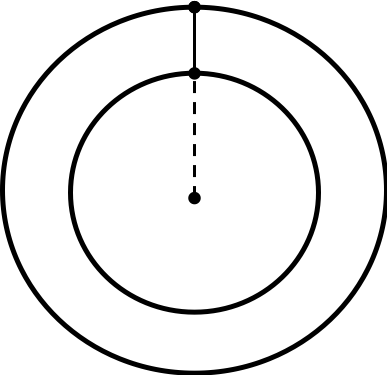
\includegraphics[scale=0.5]{img/circles-paradox.eps}
 %\captionsetup{labelformat=empty}
 \caption{同心大圆上任意一点都可通过半径对应到小圆上的唯一点}
 \label{fig:circles-paradox}
%\end{wrapfigure}
\end{figure}

由于这些悖论的出现,人们接受了亚里士多德的观点,采取回避的态度。伽利略发现无法解释自然数和平方数孰多孰少后说:因此我们不能说自然数构成一个集合。人们拒绝“全体自然数”这类说法,否认实无限的存在。

%\begin{figure}[htbp]
\begin{wrapfigure}{R}{0.4\textwidth}
 \centering
 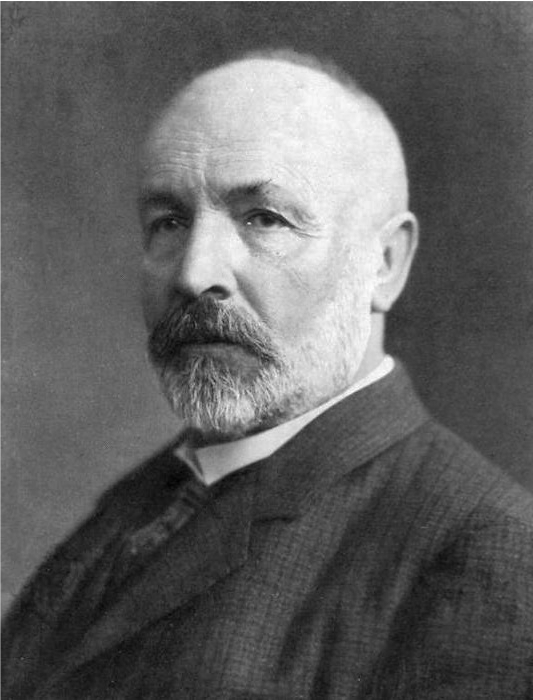
\includegraphics[scale=0.5]{img/Cantor.eps}
 \captionsetup{labelformat=empty}
 \caption{格奥尔格$\cdot$康托尔(1845-1918)}
 \label{fig:Cantor}
\end{wrapfigure}
%\end{figure}

终于,在伽利略身后两百年,德国数学家康托尔带领人们闯入了无穷王国。康托尔重新思考了陷入矛盾的一系列悖论,看起来问题的关键在于人们的常识——即整体一定大于部分。这一定是对的么?近代科学的发展一再告诉我们,人们根深蒂固用于具体事物的常识有时并不适用于更加抽象的概念。相对论挑战着人们的时空观常识——我们的所在的空间并不一定是熟悉的欧几里得空间,量子力学力学挑战着人们的因果观常识——随机性主导着量子世界。常识一旦突破,就会打开一片从未见过的新天地,从而带来巨大的认知进步。康托尔大胆地思考,如果我们接受“部分能够等于整体”的观点,通向无穷的大门就打开了。他提出“可以通过一一对应的方法来比较两个集合的大小,实无限是确实存在的概念。”

为了比较两个集合的大小,康托尔定义:如果能够建立集合$M$和集合$N$中元素的一一对应关系,那么这两个集合具有相同的基数(cardinal number),或者说它们是“等势”的\footnote{可以回想第三章中我们介绍的“同构”概念。}。对于有限集,显然这一结论是正确的,推广到无限集,根据这一定义,全体偶数和全体自然数一样多!完全平方数和自然数一样多,小圆上的点和大圆上的点也是一样多……甚至康托尔的挚友戴徳金干脆这样定义无穷集合:如果一个集合的部分和整体可以具有相同的基数,那么这个集合是无穷集合。

% Cardinality vs. cardinal number

\subsection{无穷王国的花园}

让我们来欣赏一下康托尔为我们打开的无穷王国中的花园。数学家希尔伯特为了帮助人们理解康托尔的无穷集合概念,在1924年的国际数学家大会上,讲了这样的一个故事。

有一个神奇的旅馆,拥有无穷多的房间。在旅游旺季的时候,旅馆住满了客人,已经满员了。这一天晚上,又来了一名客人。要是一般的旅馆,就只能拒绝这个新客人入住,让他另找一家了。旅店经理希尔伯特说:“没问题,住得下。”他于是指挥客人,让1号房间的客人搬到2号房间去,2号房间的客人搬到3号房间去,3号房间的客人搬到4号房间去……每个房间的客人都搬到下一个房间去。这样就空出了1号房间给新来的这位客人。

故事没有结束。第二天,旅店迎来了一个神奇的旅游团,不同于普通的旅游团,它有无穷多个游客。酒店经理希尔伯特又说:“没问题,住得下。”他指挥房间里的客人。让昨天住进1号房间的那位新客人搬到2号房间去,让2号房间的客人搬到4号房间去,让3号房间的客人搬到6号房间去……每个房间的客人都搬到房间号2倍的那个房间去。由于酒店有无穷多的房间,所以这样一搬,2, 4, 6, ...这些偶数房间住着原来的客人。而1, 3, 5, ...这些奇数房间空出来,有无穷多间。刚好可以让旅游团的人一人一间住下。

故事更加曲折了。到了第三天,旅馆门前车水马龙,来了无穷多的神奇旅游团,每个旅游团都有无穷多个游客。希尔伯特的无穷旅馆还能住下么?在揭晓答案之前,我们先回顾一下前两天的故事。

\begin{figure}[htbp]
%\begin{wrapfigure}{R}{0.4\textwidth}
 \centering
 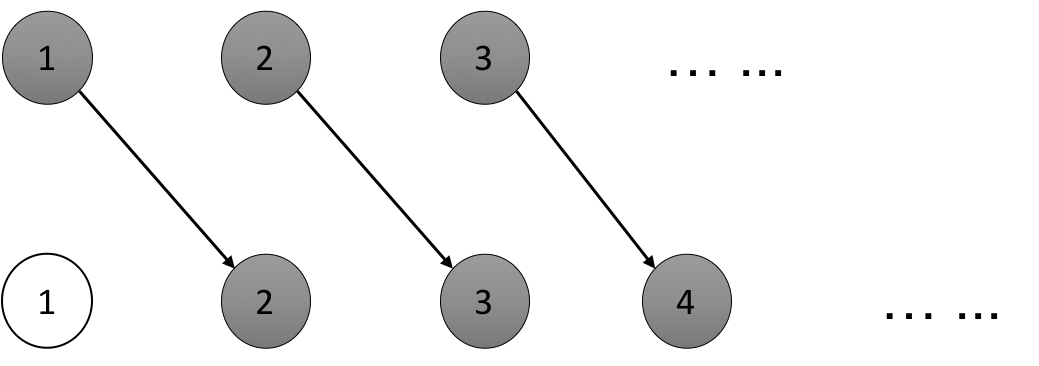
\includegraphics[scale=0.4]{img/Hilbert-hotel-1.eps}
 %\captionsetup{labelformat=empty}
 \caption{希尔伯特无穷旅馆的第一天}
 \label{fig:Hilbert-hotel-1}
%\end{wrapfigure}
\end{figure}

如图\ref{fig:Hilbert-hotel-1}所示,在第一天的故事中,我们让每个客人搬到下一个房间去,从而空出1号房间。实际上,这建立了图中上下两行灰色圆形之间的一种对应关系$n \leftrightarrow n+1$。这告诉我们一个有趣的事实,无穷加上1还是无穷。不仅如此,即使来了有限多名$k$位新客人,我们可以重复这一“腾笼换鸟”的过程$k$次,仍然能够让满员的宾馆住下他们。这相当于:

\bean
\infty + 1 = \infty \\
\infty + k = \infty \\
\eean

\begin{figure}[htbp]
%\begin{wrapfigure}{R}{0.4\textwidth}
 \centering
 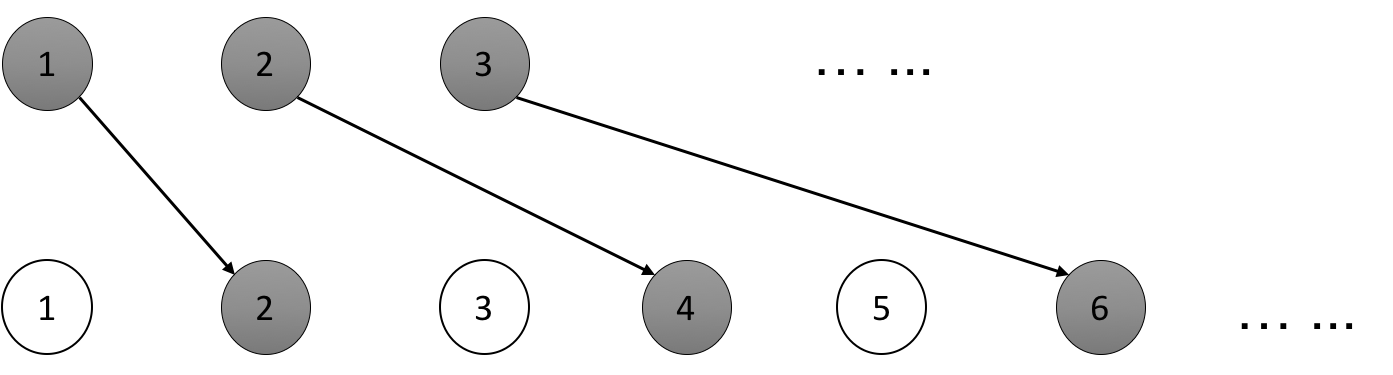
\includegraphics[scale=0.4]{img/Hilbert-hotel-2.eps}
 %\captionsetup{labelformat=empty}
 \caption{希尔伯特无穷旅馆的第二天}
 \label{fig:Hilbert-hotel-2}
%\end{wrapfigure}
\end{figure}

第二天的故事如图\ref{fig:Hilbert-hotel-2}所示,我们实际上建立了自然数到偶数间的一一映射,从而空出了无穷多间奇数房间,而这些空房间又和旅游团的无穷多位客人之间建立了一一映射,这恰好是奇数到自然数间的一一映射。第二天的故事告诉我们,无穷加上无穷仍然是无穷。

\[
\infty + \infty = \infty
\]

尽管符号相同,我们还是不禁会问,等号左边的无穷和等号右边的无穷是相同的么?无穷之间还能再比较大小么?我们稍后会看到,正是这个问题,导致了康托尔的进一步研究。在希尔伯特旅馆的问题中,这些无穷之间都可以建立一一对应关系,因此它们是“相等”的。我们把和自然数一一对应的无穷叫作可数无穷。

要想解决希尔伯特旅馆第三天的问题,我们需要思考能否在无穷个无穷旅游团和无穷个房间之间建立一一对应。有人说,可以先让第一个旅游团依次入住1, 2, ...号房间,然后让第二个旅游团的第一个客人住在$\infty + 1$号房间,第二个客人住$\infty + 2$号房间……以此类推。但是这样的思路是行不通的,我们事先并不知道究竟是房间多,还是客人多。考虑安排客人的过程,第二个旅游团的第一个客人永远不知道第一个旅游团何时入住完,从而确定自己应该搬入的房间。与之相反,在第一天的故事中,一旦1号房间的客人搬入2号房间,新客人就可以立即入住了。尽管每个客人都依次搬入下一个房间是一个无穷无尽的过程。第二天的故事中也是如此,原1号房间的客人搬到2号房间的同时,旅游团中的第1个客人就可以搬入空出来的1号房间了,接下来原2号房间的客人搬到4号房间,原3号房间的客人搬到6号房间,此时旅游团中的第2个客人就可以搬入3号房间了……

\begin{figure}[htbp]
\centering
\begin{tikzpicture}
  \draw[step=1, very thin, gray] (0, 0) grid (5, 5);
  \draw[->] (-0.25, 0) -- (6, 0) coordinate (x axis);
  \draw[->] (0, -0.25) -- (0, 6) coordinate (y axis);
  \foreach \x in {0, 1, 2, 3, 4, 5}
    \path (\x, -0.25) node[left] {\x};
  \foreach \y in {1, 2, 3, 4, 5}
    \path (-0.25, \y) node[below] {\y};
  \foreach \i / \x / \y in {0/0/0, 1/1/0, 2/0/1, 3/0/2, 4/1/1, 5/2/0, 6/3/0, 7/2/1, 8/1/2, 9/0/3, 10/0/4}{
    \path (\x, \y) coordinate (N\i);
    \fill (N\i) circle (1pt) node[above right=3pt of N\i] {\i};
  }
  \foreach \i in {0,...,9} {
    \pgfmathsetmacro{\j}{\i+1}
    \draw[-latex, thick] (N\i) to (N\j);
  }
\end{tikzpicture}
\caption{对无穷个无穷的一种编号方案}
\label{fig:NNtoN}
\end{figure}

图\ref{fig:NNtoN}给出了一种编号方案。为了方便,我们让每个旅游团的第一个客人编号为0,第二个客人编号为1,第三个客人编号为2……,我们把已经在旅馆中入住的客人编号为0号旅游团,新来的第一个旅游团编号为1号团,第二个旅游团编号为2号团……在这个图中,每个客人就对应无穷伸展的方格子中的一个点。同样我们让旅馆的房间号也从0开始。

现在我们按照这个顺序安排入住:第0号团的第0号客人入住0号房间,第0号团的第1号客人入住1号房间,第1号团的第0号客人入住第2号房间,第2号团的第0号客人入住3号房间,第1号团的第1号客人入住4号房间……这样按照图中往返画“之”字形,就可以逐一、并且毫无遗漏地安排每个客人入住。我们在无穷个旅游团的每个客人和无穷个房间之间建立了一一映射。希尔伯特的旅馆神奇地容纳了“二维”的无穷。

\begin{Exercise}
\Question{我们用图\ref{fig:NNtoN}建立了房间和任意旅游团的客人间的一一映射。第$i$号旅游团的第$j$号客人应该入住几号房间?第$k$个房间里住了哪号旅游团的哪位客人?}
\Question{希尔伯特旅馆第三天的故事的解法并不唯一,图\ref{fig:PWW-NNtoN}是《无需语言的证明》一书的封面。试根据此图给出另一种编号方案?
\begin{figure}[htbp]
 \centering
 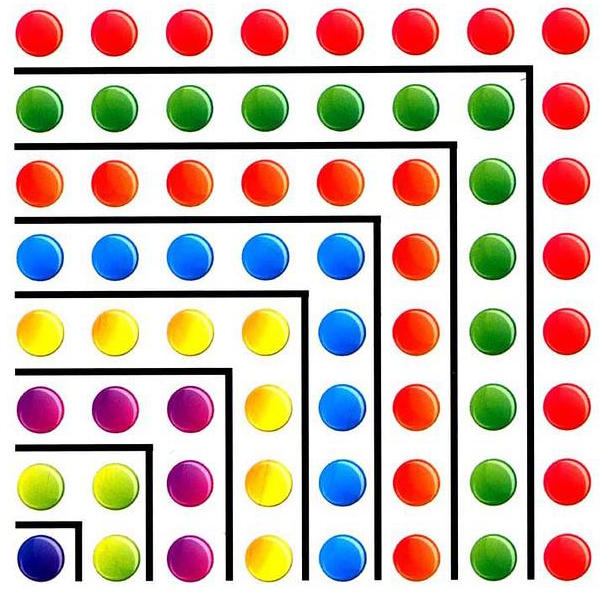
\includegraphics[scale=0.2]{img/PWW.eps}
 \caption{《无需语言的证明》封面局部}
 \label{fig:PWW-NNtoN}
\end{figure}
}
\end{Exercise}

\subsection{一一对应与无穷集合}

从希尔伯特旅馆的故事中,我们看到一一对应的概念对于研究无穷的重要性。如果能建立两个集合间的一一对应关系,则它们具有相同的基数。进一步我们可以用一一对应对集合进行分类。我们曾经在第三章介绍过相应的概念。具体说就是在两个集合$A$和$B$之间建立一个映射$A \arrowto{f} B$,使得$A$中的每个元素$x$,都可以通过映射$x \mapsto y = f(x)$,与$B$中的元素$y$关联起来。对于集合,我们也称映射$f$为函数。$y$叫作$x$的像,而$x$叫作原像。如果原像是唯一的,我们称这样的映射为\textbf{单射};如果$B$中的任何$y$都存在原像,我们称这样的映射为\textbf{满射}。既是单射又是满射的映射称为一一映射。图\ref{fig:bijection}描述了两个有限集合间的一个一一映射。

\begin{figure}[htbp]
%\begin{wrapfigure}{R}{0.4\textwidth}
 \centering
 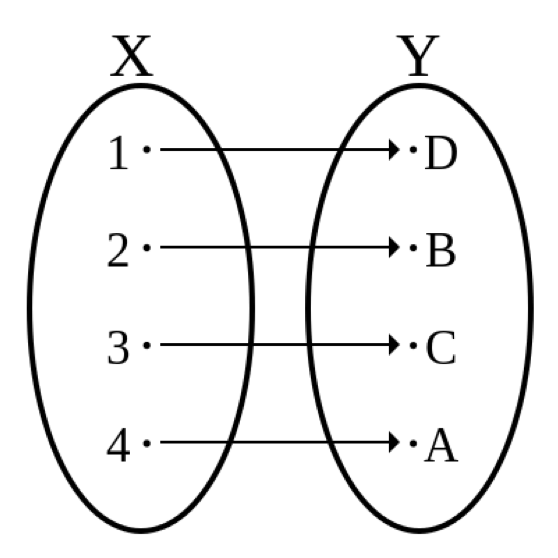
\includegraphics[scale=0.4]{img/bijection.eps}
 %\captionsetup{labelformat=empty}
 \caption{集合间的一一对应}
 \label{fig:bijection}
%\end{wrapfigure}
\end{figure}

希尔伯特的无穷旅馆系列故事既让人感到神奇和震惊,也让人困惑。自然数不仅和它的无穷子集奇数和偶数同样多,并且一维的自然数$n$和二维的自然数对$(m, n)$也同样多。这意味着什么呢?康托尔发现,他可以从自然数开始,利用一一对应,扩展出一系列的无穷集合。我们来看一下这些例子。

\begin{enumerate}
\item \textbf{整数}。如果我们建立这样的一一对应:

\begin{tabular}{ccccccccc}
0 & 1 & -1 & 2 & -2 & ... & $n$ & $-n$ & ... \\
$\updownarrow$ & $\updownarrow$ & $\updownarrow$ & $\updownarrow$ & $\updownarrow$ & & $\updownarrow$ & $\updownarrow$ & \\
0 & 1 &  2 & 3 &  4 & ... & $2n - 1$ & $2n$ & ... \\
\end{tabular}

这样就把整数和自然数对应起来。换一种角度,我们实际上用奇数对应了全部正整数,用偶数对应了零和全部负整数。这说明全体整数和自然数一样多。换言之,我们可以用自然数构造整数。
\item \textbf{有理数}。我们知道,有理数又叫作可比数,可以写成$p/q$的形式,其中$q \neq 0$。回想希尔伯特无穷旅馆第三天的的故事,用同样的方法,我们可以在任何数偶$(p, q)$和自然数之间建立一一映射。我们只要稍作修改就可以建立有理数$p/q$和自然数间的一一对应。先不考虑负数的情形,每当遇到第二个数$q$等于0就跳过,如果$p/q$不是既约分数(含有公因子)就跳过。然后我们复用扩展整数的方法,再把负有理数包含进来,这样就从自然数构造出了全体有理数。例如下表给出了前几个自然数到有理数的对应关系:

\begin{tabular}{cccccccccc}
0 & 1 & 2 & 3 & 4 & 5 & 6 & 7 & 8 & ... \\
$\updownarrow$ & $\updownarrow$ & $\updownarrow$ & $\updownarrow$ & $\updownarrow$ & $\updownarrow$ & $\updownarrow$ & $\updownarrow$ & $\updownarrow$ & \\
0 & 1 & $\dfrac{1}{2}$ & $-\dfrac{1}{2}$ & -1 & -2 & $-\dfrac{2}{3}$ & $-\dfrac{1}{3}$ & $\dfrac{1}{3}$ & ... \\
\end{tabular}

这说明自然数和有理数同样多。

\index{代数数}
\item \textbf{代数数}。所谓代数数,是指可以通过代数方程求解出的数。简单说,就是可以通过有限次加减乘除、乘方开方得到的数。因此$\sqrt{2}$和$1 \pm \sqrt{3}i$是代数数,而$\pi, e$都不是代数数。因此,任意给定一个整系数代数方程:
\[
a_0 x^n + a_1 x^{n-1} + ... + a_n = 0
\]
其中$a_0, a_1, ... a_n$都是整数,且$a_0 \neq 0$。它的所有根都是代数数。我们构造一个正整数:
\[
h = n + |a_0| + |a_1| + ... + |a_n|
\]
也就是次数和方程系数绝对值的和。我们称$h$为方程的高。因此,对于任意的代数方程,高$h$总是一个确定的自然数。反之,给定一个自然数$h$,对应的方程却不止一个。例如:$x - 3 = 0, x^3 + 1 = 0, x^3 - 1 = 0, x^2 + x + 1 = 0, x^2 - x + 1 = 0$的高都是4。但是对于固定的$h$,以它为高的代数方程只有有限多个。因此我们可以把所有的代数方程枚举出来,先枚举$h=1$的代数方程,在枚举$h=2$的代数方程……如此下去,就可以把所有的代数方程都枚举出来。当然,高同样的方程可以按任意顺序排列。根据高斯证明的代数基本定理,方程根的个数等于它的次数$n$。如果考虑重根,则不同的根不超过$n$。于是高为$h$的代数方程的根只有有限个。现在我们就可以枚举所有代数数了。

首先把高$h=1$的代数方程(只有一个$x = 0$)的根枚举出,就是0,再把高为2的方程的所有根枚举出。注意,不同方程的某个根可能是相等的,如果我们遇到某个根,在此前已经枚举过了,我们就将它跳过。这样就把代数数同自然数一一对应起来了。因此,自然数和代数数同样多。换言之,我们可以通过自然数扩展出全部代数数。
\end{enumerate}

接下来我们遇到了难题,我们能否从自然数扩展到实数?不仅包括普通的无理数,还包括$\pi$,$e$这样的超越数?解决这个难题的是康托尔和戴徳金。再进一步介绍这些伟大的成果之前,让我们先了解一下这两位数学家。

\subsubsection{康托尔与戴徳金}

%\begin{figure}[htbp]
\begin{wrapfigure}{R}{0.4\textwidth}
 \centering
 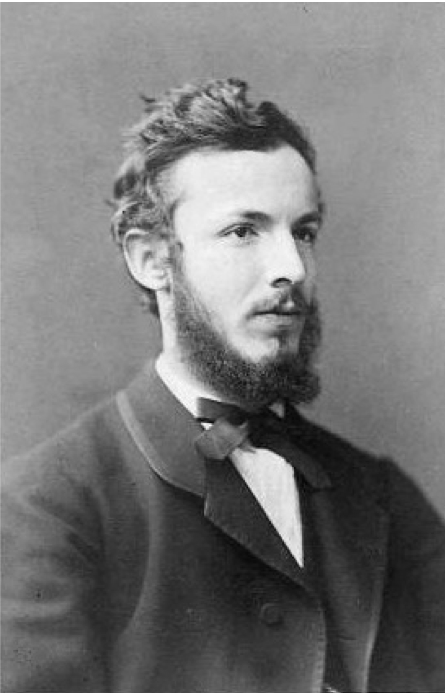
\includegraphics[scale=0.5]{img/Cantor-1870.eps}
 \captionsetup{labelformat=empty}
 \caption{康托尔摄于1870年的照片}
 \label{fig:Cantor-1870}
\end{wrapfigure}
%\end{figure}

\index{康托尔}
康托尔是德国数学家,集合论的创始人。1845年3月3日生于俄罗斯圣彼得堡,他一生的大部分时间是在德国度过的。康托尔的父亲是具有犹太血统的丹麦商人,母亲出身艺术世家。1856年举家迁居德国的法兰克福。尽管康托尔较早就显示出了数学才能,他的父亲却希望他成为一名工程师,因为这样更容易求职和谋生。直到17岁时,康托尔的父亲才逐渐意识到不应该把自己的意见强加给儿子。他得到父亲的允许,进入大学学习数学。康托尔给父亲回信道:“你自己也能体会到你的信使我多么高兴。这封信确定了我的未来……现在我很幸福,因为我看到如果我按照自己的感情选择,不会使你不高兴。我希望你能活到在我身上找到乐趣,亲爱的父亲;从此以后我的灵魂,我整个人,都为我的天职活着;一个人渴望做什么,凡是他的内心强制他去做的,他都会成功!”\cite{HanXueTao16}

1862年,康托尔进入苏黎世大学,1863年转入柏林大学攻读数学和神学,受教于大数学家库默尔、魏尔斯特拉斯、和克罗内克。1866年曾去哥廷根学习一个学期。1867年他在库默尔的指导下以解决整系数不定方程的论文获得博士学位。当时的数学界正在魏尔斯特拉斯的领导下进行着重建微积分严密基础的运动,康托尔也很快转入这一研究方向。在工作中,他意识到必须研究作为微积分基础的实数点集,这成为了集合论研究的开端。

1872年康托尔在瑞士旅游中偶遇了数学家戴徳金。两人后来成为亲密的朋友,彼此通过信件交流,互相支持。1874年29岁的康托尔发表了关于集合论的第一篇革命性论文。康托尔开始显示他非凡的独创力。在随后的十几年中,他几乎独自一人把集合论推向深入,引领了数学中无穷的革命。在他最伟大的、最具创见的时期,康托尔却没有能得到应有的认可。他没能取得柏林大学的教授职位。他的大部分研究时光是在哈雷大学度过的。这是一所不大出名、薪金微薄的二流学院。他的成果在当时很难被理解。由于太过颠覆传统,加之无穷集合引发了一些悖论(我们将在下一章详细介绍罗素悖论),人们对集合论的基础和可靠性产生了严重的怀疑。康托尔遭到了许多人的反对,其中反对最激烈的是他的老师,柏林学派的代表人物克罗内克。克罗内克有一句名言:“上帝创造了自然数,其余都是人的工作。”他批判康托尔的无穷集合和超限数理论不是数学而是神秘主义,是一类危险的数学疯狂。他认为数学在康托尔的领导下正在走向疯人院。除了克罗内克之外,还有一些著名的数学家也对集合论发表了反对意见,包括法国著名数学家——被称为最后一个数学通才的庞加莱,他说:“我个人,而且还不只我一个人,认为重点在于,切勿引进一些不能用有限个文字去完全定义好的东西。”他把集合论当作一个有趣的“病理学的情形”来谈,并且预测说:“后一代将把集合论当作一种疾病,而人们已经从中恢复过来了”。德国数学家赫尔曼$\cdot$外尔认为,康托尔关于基数的等级观点是“雾上之雾”。克莱因也不赞成集合论的思想。施瓦兹原来是康托尔的好友,但他由于反对集合论而同康托尔断交。集合论的悖论出现之后,一些数学家开始认为集合论根本是一种病态,他们以不同的方式发展为经验主义、直觉主义、构造主义等学派,在数学的基础大战中,构成反康托尔的阵营。

于是悲剧的结局不是集合论进入了疯人院,而是康托尔进入了疯人院。1884年5月,他支持不住了,第一次精神崩溃。在他一生的随后岁月中,这种崩溃以不同强度反复发生,把他从社会上赶进精神病院这个避难所。1904年在两个女儿的陪同下,他出席了第三届国际数学家大会。会上他的精神受到严重刺激,立即被送进医院。在他生命的最后十年,他大都处于严重的抑郁状态中,并在哈雷大学的精神病诊所度过了漫长的岁月。他最后一次住进精神病院是1917年5月,直至1918年1月去世。

康托尔的集合论得到公开的承认和热情的称赞应该说首先在瑞士苏黎世召开的第一届国际数学家大会上表现出来。瑞士苏黎世理工大学教授胡尔维茨(Hurwitz,Adolf,1859-1919)在他的综合报告中,明确地阐述康托尔集合论对函数论的进展所起的巨大推动作用,这破天荒第一次向国际数学界显示康托尔的集合论不是可有可无的哲学,而是真正对数学发展起作用的理论工具。在分组会上,法国数学家阿达玛也报告康托尔对他的工作的重要作用。随着时间的推移,人们逐渐认识到集合论的重要性。希尔伯特高度赞誉康托尔的集合论“是数学天才最优秀的作品”,“是人类纯粹智力活动的最高成就之一”,“是这个时代所能夸耀的最巨大的工作”。在1900年第二届国际数学家大会上,希尔伯特高度评价了康托尔工作的重要性,并把康托尔的连续统假设列入20世纪初有待解决的23个重要数学问题之首。当康托尔的朴素集合论出现一系列悖论时,直觉主义学派的代表布劳威尔等人借此再次发难,希尔伯特用坚定的语言向他的同代人宣布:“没有任何人能将我们从康托尔所创造的伊甸园中驱赶出来”。

%\begin{figure}[htbp]
\begin{wrapfigure}{L}{0.4\textwidth}
 \centering
 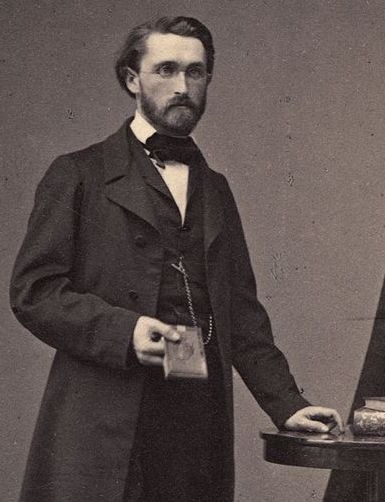
\includegraphics[scale=4]{img/Dedekind.eps}
 \captionsetup{labelformat=empty}
 \caption{理查德$\cdot$戴徳金(1831-1916)}
 \label{fig:Dedekind}
\end{wrapfigure}
%\end{figure}

\index{戴徳金}
戴徳金是德国数学家、教育家。1831年10月6日生于德国的不伦瑞克镇的一个知识分子家庭。这里也是著名数学家高斯的故乡。戴徳金的父亲为法学教授,母亲也是一位教授的女儿。1850年戴徳金到哥廷根大学师从著名的数学大师高斯研究最小二乘法和高等测量,向斯特恩学习数论基础,向韦伯学习物理,他还选修过天文学。1852年他在高斯的指导下获得博士学位,博士论文是《关于欧拉积分的理论》。在哥廷根求学期间,他还结识了黎曼、狄利克雷。在于这些世界级的数学家交流中,他获益匪浅,并逐渐萌生了用算术性质来重新定义无理数的想法。1854年戴徳金留校任代课教师。如第三章所说,他很早就在教学中讲授伽罗瓦理论并引入了域的概念。

戴徳金为人谦逊。他的许多成果并不为当时的人所知。例如在狄利克雷去世之后,戴徳金根据当时听讲的笔记整理出了《数论讲义》这一名著。尽管戴徳金在后继版本中添加了很多结论,但他却谦逊地将这本书记在了狄利克雷名下。令人遗憾的是,这种做法对其职业生涯造成了影响。他没有能获得哥廷根大学的终身教席,而是去了一家比较小的技术大学(\cite{Stepanov}第119页)——在他家乡不伦瑞克的高等工业学院。

事物总是两面性的,在不伦瑞克,戴徳金感觉自己有从事数学研究的充分时间与足够的自由。1888年,戴德金提出了算术公理的完整系统,其中包括完全数学归纳法原理的准确表达方式。戴德金的主要成就是在代数理论方面。他研究过任意域、环、群、结构及模等问题,并在授课时率先引入了环(域)的概念,并给理想子环下了一般定义,提出了能和自己的真子集建立一对应的集合是无穷集的思想。在研究理想子环理论过程中,他将序集(置换群)的概念用抽象群的概念来取代,并且用一种比较普通的公式(戴德金分割概念)表示出来,直接影响了后来皮亚诺的自然数公理的诞生。是最早对实数理论提出了许多论据的数学家之一。现今数学上的许多命题和术语,如群、环、域、结构、模、理想、函数、定理等,都是与他的名字联系在一起的。

戴徳金于1916年2月12日去世。说到他的去世,有一则趣闻。有一天,戴徳金发现托博纳写的《数学家传记》中,赫然写到:1897年9月4日戴徳金去世。出于纠正这个错误的想法,他给传记的编辑写去了一封信:“根据我本人的日记,我在这一天非常健康,而且与我的午餐客人,尊敬的朋友康托尔一起谈论着一些趣事,过得非常愉快。”\cite{HanXueTao16}

即使在当代,数学界对于康托尔和戴徳金学派的观点仍存在分歧。迪厄多内在1980年代仍然认为戴徳金的工作引起了不必要的混乱。更不用说二十世纪之初的激烈分歧和争执了。我们今天看到的大多数传记和评论往往过于批判责备克罗内克、布劳威尔及其代表的直觉主义,而同情康托尔的不幸遭遇,并热情赞颂无穷集合和超限数的革命性创造。作为今天理性的读者,我们建议大家独立思考,而不要被一边倒的观点左右。克罗内克和康托尔都是虔诚的宗教信徒,克罗内克对数学哲学有着强烈的信念,试图将一切数学(从代数学到分析)算术化是他的最高愿望。他写道:“有一天人们将成功地将所有数学算术化,就是说将数学建立在最狭义的数概念的单一基础上。”他相信人们在各种数学分支中能够也必须以这种方式限定一个定义,即人们可用有限步验证它是否适用于任意已知量。同样,一个量的存在性证明只有当它包含一种方法,通过它可以实际地发现要证明存在的量时,才可被认为是完全严格的。这些正是后来重要的数学哲学流派——直觉主义学派所坚持的信念。因此,克罗内克被认为是直觉主义学派的先驱。他的这些原则也正是现代数学的重要领域——构造性数学研究的起点。他的怀疑精神对人们重新批判地检查数学的基础起了鼓舞作用。它导致了数学中两种有建设性的批判运动:有限步构造性证明与存在性证明,以及从数学中驱除不能以有限个词明确表述的定义。这些有利于人们更清楚地认识数学的本质。庞加莱的观点也是值得我们深入思考的。他在《科学与假设》这本书中阐述了他的哲学思想。他认为公理是一种约定。在思考物理学的基本定义,如力的定义时他说,如果一个定义不能让我们去测量它,这个定义就没有任何用处。庞加莱的思想直接影响了爱因斯坦和相对论。

\subsubsection{利用(可数)无穷定义斐波那契数列和哈明数列}

有些编程环境,所有的求值默认都是惰性的,在这样的环境中,我们甚至可以直接拿潜无穷流进行复杂的计算。例如下面是另一种自然数的定义方法:

\[
N = 0 : map(succ, N)
\]

它的含义是,$N$是一个潜无穷,代表自然数。第一个自然数是0,从第二个自然数开始,后面每个自然数,都等于前一个自然数的后继。如同下面的表格:

\begin{tabular}{|r|r|l|l|l|l|}
\hline
                 & $N$: & 0 & 1 & 2 & ... \\
\hline
                 & $map(succ, N)$: & $succ(0)$ & $succ(1)$ & $succ(2)$ & ... \\
\hline
$0 : map(succ, N)$: & 0 & 1 & 2 & 3 & ... \\
\hline
\end{tabular}

例如下面的代码先定义了自然数的潜无穷,然后取出其中的前10个自然数:

\lstset{frame=single}
\begin{lstlisting}
nat = 0 : map (+1) nat

take 10 nat
[0,1,2,3,4,5,6,7,8,9]
\end{lstlisting}

类似地,我们也可以用潜无穷定义斐波那契数列。假设$F$是全体斐波那契数列,我们知道它的第一个元素是0,第二个是1,后面每个斐波那契数都是前面两个的和。我们可以仿照自然数的例子列出下面的表格:

\begin{tabular}{|r|r|l|l|l|l|l|l|l|l|}
\hline
  & $F$:  & 0 & 1 & 1 & 2 & 3 & 5 & 8 & ... \\
\hline
  & $F'$: & 1 & 1 & 2 & 3 & 5 & 8 & 13 & ... \\
\hline
0 & 1     & 1 & 2 & 3 & 5 & 8 & 13 & 21 & ... \\
\hline
\end{tabular}

其中第一行为全体斐波那契数。第二行为去掉一个元素后的全体斐波那契数。也可以这样想:把第一行向左移动一格就得到了第二行。第三行最有趣,把前两行每列加起来,我们就又得到了全体斐波那契数,只不过缺了最开始的两个数0和1。所以把它们两个补在第三行的最左边。把第三行翻译过来就是斐波那契数的潜无穷流定义:

\[
F = \{0, 1\} \cup \{ x + y | x \in F, y \in F'\}
\]

或者写成代码:
\begin{lstlisting}
fib = 0 : 1 : zipWith (+) fib (tail fib)
\end{lstlisting}

\index{正规数} \index{哈明数}
我们再给出一个稍微复杂些的例子,数学上把只含有2、3、5这三个因子组成的自然数叫作正规数。在计算机科学中,也常常叫作哈明数以纪念美国数学家,图灵奖获得者理查德$\cdot$哈明(1915-1998)。前几个哈明数如下:

\[
1, 2, 3, 4, 5, 6, 8, 9, 10, 12, 15, 16, 18, 20, 24, 25, 27, 30, 32, 36, 40, 45, 48, 50, 54, 60, ...
\]

写一个计算机程序来产生哈明数并不简单,然而利用无穷流,我们可以得到一个直观高效的解法。假设全体哈明数的潜无穷流为$H$。我们知道第一个哈明数是1,后面的哈明数可以这样构造,我们把$H$中的每个数都乘以2,仍然是哈明数,记作$H_2 = \{ 2x | x \in H \}$,类似地我们可以定义$H_3 = \{ 3x | x \in H \}$和$H_5 = \{ 5x | x \in H \}$,如果把这三个新序列中的数,从小到大合并起来,去掉重复的,并且在前面补充上1,就又得到了全体哈明数。

\[
\begin{array}{rcl}
H & = & \{ 1 \} \cup H_2 \cup H_3 \cup H_5 \\
  & = & \{ 1 \} \cup \{ 2x | x \in H \} \cup \{ 3x | x \in H \} \cup \{ 5x | x \in H \} \\
\end{array}
\]

其中$\cup$的含义就是从小到大,去掉重复、合并两个无穷序列$X = \{x_1, x_2, ...\}$和$Y = \{y_1, y_2, ...\}$:

\[
X \cup Y =
\begin{cases}
x_1 < y_1 : & \{x_1, X' \cup Y \} \\
x_1 = y_1 : & \{x_1, X' \cup Y' \} \\
x_1 > y_1 : & \{y_1, X \cup Y' \} \\
\end{cases}
\]

写成代码就是:

\begin{lstlisting}
ham = 1 : map (*2) ham # map (*3) ham \# map (*5) ham
  where xxs@(x:xs) # yys@(y:ys)
    | x==y = x : xs # ys
    | x<y  = x : xs # yys
    | x>y  = y : xxs # ys

ham !! 1000000
519312780448388736089589843750000000000000000000000000
000000000000000000000000000000
\end{lstlisting}

\lstset{frame=none}

\subsection{可数无穷与不可数无穷}
\index{可数集}
迄今为止,我们用自然数构造了整数、有理数、和包含部分无理数的代数数。它们都和自然数之间存在一一映射,或者说和自然数一样多。我们把和自然数等势的无穷集合叫作可数无穷。是不是所有的无穷集合都是可数的呢?是否存在更大的无穷呢?1873年11月29日康托尔给戴徳金的一封信中提到了这个问题:“取所有的自然数集合,记为$N$,然后考虑所有实数的集合,记为$R$。简单来说,问题就是两者是否能够对应起来,使得一个集中的每一个体只对应另一集中一个唯一的个体?乍一看,我们可以说答案是否定的,这种对应不可能,因为前者由离散的部分组成,而后者则构成一个连续统。但从这种说法里我们什么也得不到。虽然我非常倾向认为这两者不能有这样的一个一一对应,但是我找不出理由,我对这事极为关注,也许这理由非常简单。”

\index{对角线证明}
一个星期后的12月7日,在写给戴徳金的信中,康托尔自己回答了这个问题,他发现实数集合不能和自然数集合构成一一对应。这一天可以看作是集合论的诞生日。康托尔曾经给出过两个证明,其中第二个证明最为脍炙人口,就是大名鼎鼎的“对角线证明”。

康托尔首先使用反证法,假设区间$(0, 1)$上的全部实数是可数的,可以和自然数一一对应。那么就可以把这个区间里的全部实数列出来,形成一个序列$a_0, a_1, a_2, ..., a_n, ...$。现在将这个序列中的每个实数都表示成小数形式。如果是无理数,它的小数形式是无限不循环的;如果是除不尽的分数,则其小数形式是无限循环的,例如$\dfrac{1}{3} = 0.333...$;如果能够除尽,我们就在后面补无穷多个零,例如$\dfrac{1}{2} = 0.5000...$。于是实数区间$(0, 1]$中的所有实数可以排成下面的序列:

\[
\begin{array}{l}
a_0 = 0.a_{00}a_{01}a_{02}a_{03}...\\
a_1 = 0.a_{10}a_{11}a_{12}a_{13}...\\
a_2 = 0.a_{20}a_{21}a_{22}a_{23}...\\
a_3 = 0.a_{30}a_{31}a_{32}a_{33}...\\
... \\
a_n = 0.a_{n0}a_{n1}a_{n2}a_{n3}...\\
... \\
\end{array}
\]

有一点我要提醒一下读者:$a_0, a_1, a_2, ...$并不一定是按照大小次序排列的。现在构造一个数$b = 0.b_0b_1b_2b_3...b_n...$,使它的第$n$位数字$b_n \neq a_{nn}$。为了做到这一点,我们可以规定一个很简单的规则,例如若$a_{nn} \neq 5$,就让$b_n = 5$,否则就让$b_n = 6$,即:

\[
b_n = \begin{cases}
5 & : a_{nn} \neq 5 \\
6 & : a_{nn} = 5 \\
\end{cases}
\]

这样构造出来的数$b$一定不等于上述序列中的任何一个数。因为至少它们的第$n$位数字不相同。也就是对角线上的数字至少不同。我们把对角线上的数字写成黑体,这样就很明显了。

\[
\begin{array}{l}
a_0 = 0.\pmb{a_{00}}a_{01}a_{02}a_{03}...\\
a_1 = 0.a_{10}\pmb{a_{11}}a_{12}a_{13}...\\
a_2 = 0.a_{20}a_{21}\pmb{a_{22}}a_{23}...\\
a_3 = 0.a_{30}a_{31}a_{32}\pmb{a_{33}}...\\
... \\
a_n = 0.a_{n0}a_{n1}a_{n2}a_{n3}...\pmb{a_{nn}}...\\
... \\
\end{array}
\]

我们此前假设$(0, 1)$间的所有实数都被逐一列出了,无一遗漏。$b$显然属于这一区间,但它却不等于任何一个$a_i$。这说明我们假设的一一映射遗漏了$b$,导致了矛盾,所以假设不成立,我们无法把这一区间的所有实数和自然数之间构造一一映射。由于利用了对角线上的数字都不相等的这一事实,这一证法称作康托尔对角线证明。

有人说,把$b$加进$a_0, a_1, a_2, ...$中去不就可以了么?假设$b$加进去后,处于第$m$个位置,我们仍然可以再次构造一个新数$c$,只要让它的第$m$位不等于$b_m$就又出现了一个没有包含的数。

\index{不可数集}
这一证明简单、直观。它揭示了一个惊人的事实:$(0, 1)$间的实数集是不可数的!它是我们发现的第一个比自然数集更大的无穷集合\footnote{柯朗在《什么是数学》中给出了一个更为直观的几何证明。假设单位线段(0, 1)之间的点能排成可数的序列$a_1, a_2, a_3, ...$我们用一个长1/10的区间盖住$a_1$点,用长1/100的区间盖住$a_2$点……用长$1/10^n$的区间盖住$a_n$点,如此下去,则(0, 1)这一单位线段将完全被长为1/10, 1/100, 1/1000……的子区间(可能相互重叠)完全盖住。但这些子区间的长度总和为等比数列$1/10 + 1/100 + 1/1000 + ... = 1/9 < 1$,让总长度为1/9的区间覆盖长度为1的线段是不可能的。所以假设错误,线段上的点是不可数的\cite{Courant1969}。}。接下来,我们构造一个一一映射:$y = \pi x - \dfrac{\pi}{2}$。它把区间$(0, 1)$中的每个实数,映射到区间$(-\dfrac{\pi}{2}, \dfrac{\pi}{2})$中,无一遗漏。因此我们立即得知这一区间内的实数集是不可数的。接下来,我们压上最后一根稻草。再构造一个一一映射:$ y = tan(x)$。它把区间$-\dfrac{\pi}{2}$到$\dfrac{\pi}{2}$中的每一个实数,无一遗漏地映射到了全体实数集上\footnote{还有一种几何方法可以将单位线段一一映射到全体实数上。我们将单位线段弄弯成为长度为1的半圆弧,然后在圆外画一条无限长的直线L。现在从圆心到L上任意一点P的连线必然与圆弧相交于一点Q。这样就形成了一一映射。}。康托尔得到了他的重要结论:实数集不再是可数集,它是比可数集更高等级的无穷。康托尔称之为不可数集,记作$C$。

这自然让人联想到线段上的点。在欧几里得的《几何原本》中,点被定义为没有大小的部分,而直线被认为由点组成。根据希帕索斯的发现,我们知道直线上存在无理数。或者说有理数不能够填充直线。而实数是可以填充线段的。我们在下一节中,还会介绍戴徳金分割,从而给出实数的严密化定义。上面的证明告诉我们,单位长度线段上的点,和任何长度线段上的点,以及无限长的直线上的点,也就是数轴上稠密的点是一样多的。都是不可数集。同心圆上的点也是同样多的,它们也都是不可数集。

同样令人吃惊的是无理数与有理数多少的比较。直观上思考,任何两个有理数之间,存在着无穷多的无理数;任何两个无理数之间,也存在着无穷多的有理数,我们会觉得无理数和有理数应该一样多。然而康托尔的结论告诉我们,有理数是可数的,而无理数是不可数的。这说明无理数远远多于有理数。再进一步,我们前面证明了代数数是可数的,这说明像$\pi, e$这样的超越数是不可数的,它们要远远多于代数数。

在希尔伯特无穷旅馆第三天的故事中,我们发现一维的可数无穷可以和二维的无穷多格子点对应起来。并以此为基础证明了有理数是可数无穷。但是一维线段上代表实数的点和二维平面上的点谁多谁少?还是同样多呢?1874年1月,康托尔在写给戴徳金的信中提出了这个问题。他几乎肯定的觉得,二维正方形比一维的线段包含更多的点。但是却没能给出证明。时光匆匆过了四年之后,康托尔惊奇地发现,他此前结论是错误的,并且找到了一个有趣的一一对应。1877年6月他写信给戴徳金,请审查他的证明。在信中,康托尔说出了本章开头那句著名的话:“我看到了,但我不相信。”

我们接下来看看这个一一对应是如何展示“一沙一世界”的奇观的。我们面对的两个无穷点集一个是单位正方形

\[
E = \{ (x, y) | 0 < x < 1, 0 < y < 1\}
\]

另一个是单位线段$(0, 1)$。取单位正方形内的任意一个点$(x, y)$,然后把$x$和$y$都表示成无穷小数(如果是有限小数,比如0.5,就写成0.4999...,请参考本节习题)。现在把$x, y$的小数部分分成一组一组的,每组都终止在第一个非0数字上。例如:

\[
\begin{array}{lcccccc}
x = 0.3 & 02 & 4 & 005 & 6 & ... \\
y = 0.01 & 7 & 06 & 8 & 04 & ... \\
\end{array}
\]

然后我们构造一个数字$ z = 0.3\ 01\ 02\ 7\ 4\ 06\ 005\ 8\ 6\ 04\ ...$。这个构造过程交错地从$x$和$y$的各组中取数字,无一遗漏。也就是先写下0和小数点,然后取$x$的第一组,也就是3,然后取$y$第一组,也就是数字01,然后取$x$的第二组02,接下来取$y$的第二组7……,$z$显然在单位线段内。对于单位正方形内不同的点,其小数表示$x$或$y$上必有不同的数字。因此对应的$z$也是不同的。这说明$(x, y) \mapsto z$是单射。反过来,对于单位线段上任意点$z$,我们也可以把$z$的无穷小数形式像上面那样分组,然后把奇数组取出放在0和小数点后构成$x$,把偶数组取出构成$y$。则$(x, y)$是单位正方形内的点。这说明$(x, y) \mapsto z$是满射。因而这个映射是一一映射。于是我们证明了单位长度线段内的点和二维平面上的点具有相同的基数,它们同样多,都是不可数无穷。

仿照此方法,我们接下来可以证明不仅线段和平面上的点同样多,它和三维空间中的点也同样多。甚至一般的$n$维空间中的点也和线段上的点同样多。

在康托尔以前,尽管有争议,但是人们只能区分出有限和无穷。没有人想过无穷之中还有区别。康托尔第一个向我们揭示,无穷也是可以分类的。存在着可数无穷和不可数无穷。康托尔并没有止步,接下来的问题是:存在比不可数无穷更大的无穷么?我们在寻找无穷等级的道路上走到终点了么?在展示进一步的结论前,我们先了解一下戴徳金关于实数别出心裁的定义。

\begin{Exercise}
\Question{令$x = 0.9999....$, 则$10x = 9.9999...$,做减法得$10x - x = 9$,解方程得$x = 1$。因此得到结论$1 = 0.9999...$。这一证明正确么?}
\end{Exercise}

\subsection{戴得金分割}
\index{戴徳金分割}
为了解决微积分基础的严密性问题,十九世纪的数学家们开始重新思考牛顿、莱布尼茨、雅可比、欧拉使用的一些令人困惑的概念。包括无穷小量和级数等等。经过柯西和魏尔斯特拉斯等人的工作,终于给出了严格的极限,收敛等概念。但有一个本质问题始终未得到圆满的解决。那就是实数的概念。微积分是建立在实数连续性上的。可人们仍然没有一个关于实数满意的定义。最早人们把有理数比作直线,结果发现有理数间充满了间隙,它是不完备、不连续的。而我们则把直线看作没有间隙的、完备的和连续的。直线的连续性究竟是什么意思?人们迫切需要连续性的一个精确定义。

戴徳金经过多年的思考,终于在1872年想出了一个方法——即著名的戴徳金分割。戴徳金指出,有理数具有稠密性,即任意两个有理数间,不管多么靠近,总存在着另外的有理数。但是有理数却不连续。连续的直线究竟意味着什么呢?此时让我们想象一把最锋利的“思想之刀”,在天衣无缝的直线上切下去,将它分割成两截(\cite{HanXueTao16},第196页)。

由于直线是连续的,天衣无缝的,不管多么锋利,这一刀一定落在某一点上,而不是在两点的缝隙间。(如果是有理数而非实数,这一刀可能落在某个有理数代表的点上,也可能落在两个有理数之间,比如恰好落在$\sqrt{2}$代表的位置上。)假定从点$A$的位置上把直线切开,则$A$不在左边,就在右边。二者必居其一,不会两边都有,也不会两边都没有。这是因为点不可分割、也不会消失掉。换言之,直线的连续性意味着,不管从何处将直线切成两段,总是有一段是带有端点的,而另一段没有端点。

由此,戴徳金定义了这样的一个分割$(A_1, A_2)$,$A_1$和$A_2$分别叫作下类和上类。其中下类$A_1$中的每个数都小于上类$A_2$中的任意一个数。也就是说$A_1$对应分割的左半段直线,而$A_2$对应着右半段直线。对于这样的分割,要么$A_1$中存在着一个最大数,要么$A_2$中存在着一个最小数。二者必居其一,且仅居其一。

\begin{figure}[htbp]
 \centering
 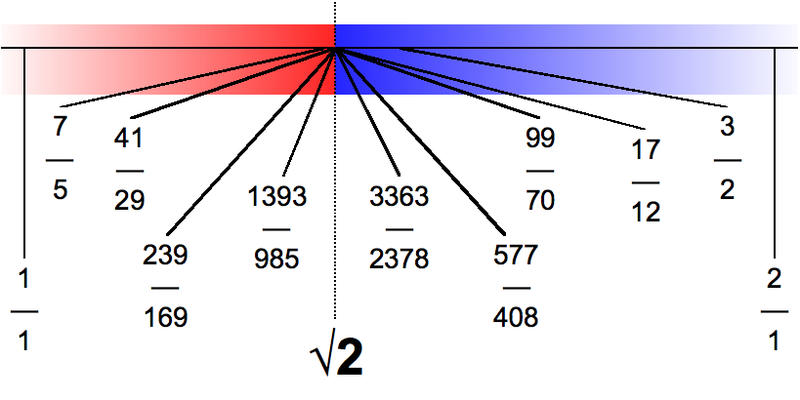
\includegraphics[scale=0.6]{img/Dedekind-cut.eps}
 %\captionsetup{labelformat=empty}
 \caption{用戴徳金分割构造的$\sqrt{2}$}
 \label{fig:Dedekind-cut}
\end{figure}

用戴徳金分割来分析全体有理数,会发现有理数是不连续的。如果$A_1$包含了所有小于等于2的有理数,$A_2$包含了所有大于2的有理数,这一分割就定义了有理数2。但是考虑这样一个反例:下类$A_1$包含所有负有理数,以及非负的,但平方小于2的有理数;上类$A_2$包含剩余的有理数。不难发现在这一分割中,下类没有最大数,同时上类没有最小数。这说明有理数间存在着缝隙,从这里砍下去,这一刀就会落空。这个划分实际上确定了一个新数$\sqrt{2}$,但它不是有理数。如图\ref{fig:Dedekind-cut}所示。

于是戴徳金得到了他的结论:有理数的每一个分割就叫作一个实数。带缝隙的分割($A_1$没有最大数,$A_2$没有最小数)叫作无理数;不带缝隙的分割($A_1$存在最大数,或$A_2$存在最小数)叫作有理数。而实数正好包含有理数和无理数。由此戴徳金分割定义了实数,直线上的每个点可以表示一个实数。戴徳金的分割概念也给出了实数连续性的依据。

从毕达哥拉斯学派的希帕索斯发现无理数到戴徳金最终给出实数的定义,时光经历了两千多年\footnote{同一年,魏尔斯特拉斯通过有界单调序列理论,康托尔通过有理数序列理论也都从有理数出发定义出无理数,从而构筑起了实数理论。可谓殊途同归。}。在戴徳金分割中,总是把数分成两个完成了的无穷整体,即无穷集合。这是对实无穷概念的运用和发展。

\subsection{超限数和连续统假设}
\index{幂集}
为了寻找更大的无穷,康托尔首先考虑了幂集。所谓幂集,就是一个集合的所有子集构成的集合。例如集合$A = \{a, b\}$,则它的幂集包含$\{\phi, \{a\}, \{b\}, \{a, b\}\}$一共四个元素。而有3个元素集合的幂集包含8个子集。一个集合中每个元素都可以被选中或者跳过以构造子集,这样具有$n$个元素的集合的幂集大小为$2^n$。显然有限集的幂集元素个数大于原集合。

\index{康托尔定理}
康托尔在1891年证明了,当推广到无限集时,这一结论也成立。所以幂集的基数总是大于原集合的基数。这一定理现在被人们称作\textbf{康托尔定理}。这一证明并不困难。读者可以参考本章的附录,了解其详细过程。有了这一定理后,就打开了寻找更大的无穷的通路了。康托尔把自然数集等可数无穷的基数称作阿列夫零,记为$\aleph_0$,阿列夫是希伯来文字母表的第一个字母。可数无穷的幂集基数记作$2^{\aleph_0}$,并且由康托尔定理有$\aleph_0 < 2^{\aleph_0}$,并且我们还可以通过幂集的幂集不断产生更大的无穷。

\be
\aleph_0, 2^{\aleph_0}, 2^{2^{\aleph_0}}, ...
\ee

\subsubsection{超限数}
\index{超限数}
康托尔把存在等级的无穷基数序列叫作超限基数。所以希尔伯特神奇旅馆中揭示的超限数计算法则就是$\aleph_0 + 1 = \aleph_0$, $\aleph_0 + k = \aleph_0 $, $\aleph_0 + \aleph_0 = \aleph_0$, ...

\index{序数}
除了用幂集来产生更高等级的无穷外,康托尔还发现了另外一种方法。为此,我们需要引入序数的归纳定义:

\begin{enumerate}
\item 0是序数;
\item 如果$a$是序数,则$a \cup \{a\}$是序数,记作$a + 1$,称作$a$的后继;
\item 如果$S$是序数的集合,也就是$S$的元素都是序数,则$\cup S$是序数;
\item 任何序数,都是通过上述1到3步获得的。
\end{enumerate}

根据这个定义,从0开始的前几个序数如下:

\[
\begin{array}{l}
0 \\
1 = 0 \cup \{0\} \\
2 = 1 \cup \{1\} = 0 \cup \{0\} \cup \{0 \cup \{0\}\} \\
3 = 2 \cup \{2\} = 1 \cup \{1\} \cup \{1 \cup \{1\}\} = ... \\
... \\
\end{array}
\]

这里$\cup S$称为集合$S$的广义并。它是由$S$的所有元素的元素组成的集合。根据序数定义的前两条,我们发现自然数0, 1, 2, 3, ..., n, ... 都是序数。令$\omega$是自然数集合,由于自然数都是序数,所以$\omega$也是一个序数的集合。我们考虑它的广义并:

\[
\cup \omega = \{0, 1, 2, ...\} = \omega
\]

根据序数的第三条定义,说明$\omega$也是一个序数,它是一个极限序数,并且是最小的无穷序数。我们把它添加到自然数的末尾就得到了一个新序列:

\[
0, 1, 2, ..., \omega
\]

从$\omega$开始,再次重复使用序数的第二条定义,又可以得到序数列:

\[
\omega + 1, \omega + 2, \omega + 3, ..., \omega + n, ...
\]

将上面两个序列合并到一起组成一个集合,记作$\omega \cdot 2$。不难发现其广义并$\cup \omega \cdot 2 = \omega \cdot 2$。所以$\omega \cdot 2$也是一个序数,并且是极限序数。从$\omega \cdot 2$开始,继续重复上述过程,我们就得到了无限伸展的无穷序数列:

\be
\begin{array}{l}
0, 1, 2, ..., n, ... \\
\omega, \omega + 1, \omega + 2, ..., \omega + n, ... \\
\omega \cdot 2, \omega \cdot 2 + 1, \omega \cdot 2 + 2, ..., \omega \cdot 2 + n, ... \\
...\\
\omega \cdot k, \omega \cdot k + 1, \omega \cdot k + 2, ..., \omega \cdot k + n, ... \\
... \\
\omega^2, \omega^2 + 1, \omega^2 + 2, ..., \omega^2 + n, ... \\
...\\
\omega^3, \omega^3 + 1, \omega^3 + 2, ..., \omega^3 + n, ... \\
...\\
\omega^\omega, \omega^\omega + 1, \omega^\omega + 2, ..., \omega^\omega + n, ... \\
...\\
\end{array}
\label{eq:countable-ordinal-nums}
\ee

除了第一行是自然数外,其它都是无穷序数,并且每行的第一个是极限序数。用这种方式得到的序数,已经远远超出人们所能想象的范围,把自然数扩展成一个无穷无尽的序数王国。但是,可以证明,这些序数都是可数序数,作为集合,竟然能够与自然数集构成一一对应。我们即将看到,还存在着不可数序数,甚至存在着一个比一个更大的无穷序数列。

我们列出的这些序数中,如果挑选一个作为可数集合的基数,用哪一个最好呢?自然会想到最小的一个极限序数$\omega$。于是这引出了基数的一般定义:

\index{基数}
\begin{definition}
设$a$是一个序数,如果对于任一序数$b$,当$b < a$时,有$b$的势小于$a$的势,则称序数$a$为基数。
\end{definition}

有这个定义,我们立即得出结论:所有自然数$n$都是基数,并且$\omega$是基数。序数$\omega$当作基数使用时,记作$\aleph_0$。即$\aleph_0 = \omega$,前面我们已经用$\aleph_0$表示可数集合的基数。

除了$\omega$外,序列(\ref{eq:countable-ordinal-nums})中其余的无穷序数都比$\omega$大,但其势却与$\omega$的势相等(都等于可数无穷)。所以根据定义,它们都不是基数。

为了获取更大的基数,为此我们将此前序列(\ref{eq:countable-ordinal-nums})中的所有序数汇集在一起组成一个集合,记作$\omega_1$。

\[
\omega_1 = \{ a | a \text{是序数,且} |a| \leq \aleph_0\}
\]

其中$|a|$表示$a$的势\footnote{严格来说,$A$的势应使用符号$\overline{\overline{A}}$,或$\#A, card(A), n(A)$。}。可以证明$\omega_1$是序数,并且是第一个不可数序数。然后我们仿照前面的方法,从$\omega_1$之后扩展无穷序数列:

\[
\omega_1, \omega_1 + 1, ..., \omega_1 \cdot 2, ..., \omega_1^2, ..., \omega_1^\omega, ...
\]

这里枚举的无穷序列都是等势的,其中最小的一个是$\omega_1$,它还满足基数的条件,这样我们就得到了第二个无穷基数$\aleph_1 = \omega_1$。仿照$\omega_1$的构造过程,我们可以再构造一个集合:

\[
\omega_2 = \{ a | a \text{是序数,且} |a| \leq \aleph_1\}
\]

这样就获得了第三个无穷基数$\aleph_2 = \omega_2$。继续进行下去,我们可以得到一系列无穷基数。概括来说,对任一序数$a$,当定义了无穷基数$\aleph_a$之后,我们可以再次构造集合:

\[
\omega_{a+1} = \{ b | b \text{是序数,且} |b| \leq \aleph_a\}
\]

由此得到比$\aleph_a$大的无穷基数$\aleph_{a+1} = \omega_{a+1}$。总之对于任一序数$a$,相应都有一个无穷基数$\aleph_a$,由此得到无穷基数组成的无穷序列:

\be
\aleph_0, \aleph_1, \aleph_2, ..., \aleph_n, ..., \aleph_{\omega}, ...
\ee

它们是从小到大排列的,并且相邻的两个阿列夫之间不再有其它的无穷基数。无穷序数和无穷基数也称为超限序数和超限基数,统称为超限数。这些越来越巨大的超限数最终归于何处呢?康托尔认为那将是上帝。

超限数一经面试,立即引发了激烈的反应。有人赞叹这是康托尔惊人的创举,开辟了前所未见的新视野。也有人认为超限数是“雾上之雾”,康托尔正在创造病态的数学。尽管存在巨大的争议,超限数是十九世纪最惊人的思想成就之一。

\subsubsection{连续统假设}
\index{连续统假设} \index{CH} \index{GCH}
康托尔发现了两种无穷基数序列,一个是幂集,另一个是超限基数:

\[
\aleph_0, 2^{\aleph_0}, 2^{2^{\aleph_0}}, ...
\]

和

\[
\aleph_0, \aleph_1, \aleph_2, ...
\]

根据上面的分析,我们知道$\aleph_1$是紧跟着可数无穷基数$\aleph_0$之后的下一个超限基数。然而根据幂集的性质,我们只知道$2^{\aleph_0}$比可数无穷基数$\aleph_0$大。但我们不知道它和$\aleph_1$的大小关系。康托尔猜测$2^{\aleph_0} = \aleph_1$,也就是在$\aleph_0$和$2^{\aleph_0}$之间不存在其它无限基数。$2^{\aleph_0}$是第一个比可数集大的超限基数。

康托尔在1847年证明了$2^{\aleph_0} = C$,也就是说,自然数的所有子集所具有的元素数正好等于实数集的元素数。因此康托尔的猜测等价于说在可数集$\aleph_0$与不可数集$C$之间不存在其它无限基数。由于通常称实数集为连续统,因此这一猜想被称为连续统假设,英文为:Continuum Hypothesis,简记为CH。

连续统假设还可以进一步推广。即考虑对于任一序数$a$,$2^{\aleph_a} = \aleph_{a+1}$是否成立。这一假设被称为广义连续统假设,简记为GCH。

康托尔在1878年的一篇论文提出了连续统假设。他一开始对证明这一猜想是比较乐观的。据说康托尔曾经说他已经成功解决了这一难题,并即将公布他的证明。但直到他1918年去世,也没有把证明公之于众。大概是发现了证明中的问题而未公开发表。康托尔晚年为此投入了大量的精力,但是长时间未能突破连续统假设,加之其它原因最终导致他陷入了抑郁,并在哈雷大学的精神病院中逝世。

1900年夏天,著名的数学家希尔伯特在巴黎召开的第二届国际数学家大会上,作了题为《数学问题》的演说。提出了23个未解决的问题,向二十世纪的数学家提出挑战。其中第一个问题就是“证明连续统假设”。可见他对这一问题的重视。

连续统问题是数学来源于几何、力学、和物理等方面现实问题的一个范例。希尔伯特认为,连续统问题来自外部世界,纯数学需要从外部世界汲取新材料,外部世界是数学的源泉。正因为连续统问题是数学中一个最基本的问题,或者说它是数学基础的问题,长期以来一直是数理逻辑和公理集合论的一个中心问题。一百多年来,虽然经过许多著名数学家的精心钻研。取得了一些重大进展,但还没有完全解决。1938年哥德尔证明了,从公理集合论的ZFC系统(策梅罗——弗兰克尔系统加上选择公理的简称,选择公理是说我们能从任一集合,包括无穷集合中选出若干元素。我们将在下一章详细介绍)推不出CH的否定。即连续统假设与ZFC系统是相容的。在哥德尔的结果之后,人们希望能够从ZF系统(ZF系统是不带有选择公理的集合论系统)内证明连续统假设。

1963年7月,美国的年轻数学家科恩创造了威力极大的力破法,解决了相反的问题,他证明了从ZFC推不出CH。这就说明了连续统假设和ZFC系统是相对独立的。有一则插曲说,科恩完成了证明后,并不能确信自己的证明(\cite{HanXueTao16},第280页)。他来到普林斯顿敲响了哥德尔的家门。当时的哥德尔正在同妄想症斗争,他仅仅打来了一条门缝,让科恩把证明塞进去。科恩则被关在了门外。两天后,哥德尔邀请科恩进屋喝茶,大师终于认可了他的证明。

综合哥德尔和科恩的结果,也就是说连续统假设在ZFC系统中是不可判定的。我们在下一章会深入介绍不可判定性。连续统假设与ZF系统的公理无关。类似的结论还发生在集合论中的选择公里上。哥德尔和科恩的结论同时也说明,选择公理在ZF系统中是不可判定的。这说明在ZF公理集合论系统中,承认选择公理可以得到一种数学;否定选择公理可以得到另一种数学。两者都是无矛盾的。同样,加上选择公理后,承认或者否定连续统假设也都可以各自发展出无矛盾的数学。这就是100多年来人们在选择公理与连续统假设的研究中获得的主要成果\cite{GCH}。

\section{无穷与艺术}

\begin{figure}[htbp]
%\begin{wrapfigure}{R}{0.5\textwidth}
 \centering
 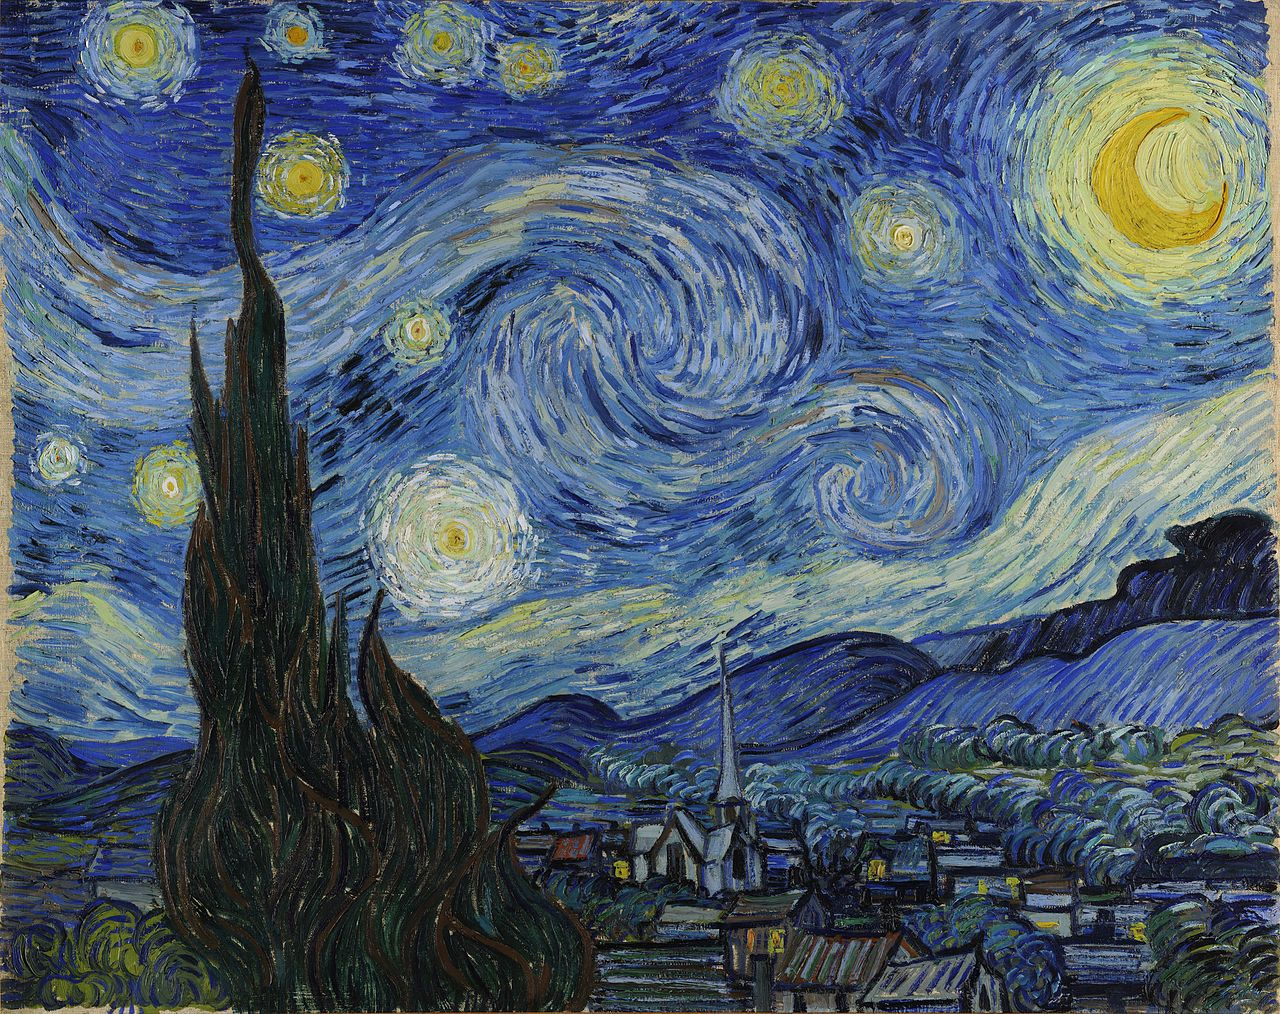
\includegraphics[scale=0.15]{img/starry-night.eps}
 \captionsetup{labelformat=empty}
 \caption{[荷]梵高《星空》1889,原作收藏于纽约现代艺术博物馆}
 \label{fig:starry-night}
%\end{wrapfigure}
\end{figure}

伴随着对无穷的思考与探索,也不断催生了关于无穷的艺术创作。人们仰视浩瀚苍穹,远眺无垠的大海,感叹自然的神秘和伟大。

在无数描绘广袤天空的作品中,荷兰后印象派艺术大师梵·高创作的《星空》可谓让人印象深刻。在这幅画中,梵高用夸张的手法,生动地描绘了充满运动和变化的星空。 整个画面被一股汹涌、动荡的蓝绿色激流所吞噬,旋转、躁动、卷曲的星云使夜空变得异常活跃,脱离现实的景象反映出梵·高躁动不安的情感和疯狂的幻觉世界。这幅画创作于1889年,当时梵·高正在阿尔勒圣雷米的一家精神病院治疗,在那驻留了108天。在入住精神病院期间,梵高创作了大量的绘画作品,共计一百五十多幅油画和一百多幅素描。而作品《星空》所描述的风景也正是精神病院所在地圣雷米。

\begin{figure}[htbp]
%\begin{wrapfigure}{R}{0.5\textwidth}
 \centering
 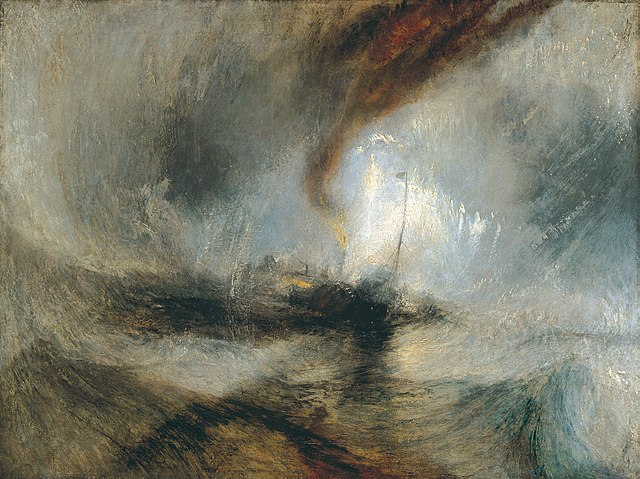
\includegraphics[scale=0.3]{img/Turner-Snow-Storm.eps}
 \captionsetup{labelformat=empty}
 \caption{透纳笔下的大海和风暴,1842。原作藏于英国泰特美术馆}
 \label{fig:Turner-Snow-Storm}
%\end{wrapfigure}
\end{figure}

英国画家透纳,在创作《暴风雪:汽船驶离港口》时,为了充分体验大海无边的威力,他让水手把自己捆在船桅上。他后来写道:“为了观察大海,我让水手们把我捆在船桅上。我那样过了四个小时,没指望能活下来。”然而,评论家们却对这幅画表示失望和怀疑,因为在这幅画中,形体和戏剧性的场面都消失了。透纳解释说,他画这幅画是为了告诉自己和别人,在惊涛骇浪的海上,暴风雪是什么样子。虽然描画的是在漩涡风暴中航行的船,但是所呈现的却是船只与风暴融为一体的画面。透纳大胆地以抽象手法表现船的形式,自由运用色彩,成功的表现出“风暴的气氛”。透纳因此被称为印象派的先驱。

对无穷的思考很快脱离了自然界中的具体事物,而上升到哲学和宗教。在托勒密的宇宙模型中,行星是嵌套在一起的同心球,最外层存在一个有界的恒星天球。到了中世纪,基督教在很大程度上吸收了亚里士多德和托勒密的学说,认为上帝创造的地球是宇宙的中心,而恒星天球是有界的。

\begin{figure}[htbp]
 \centering
 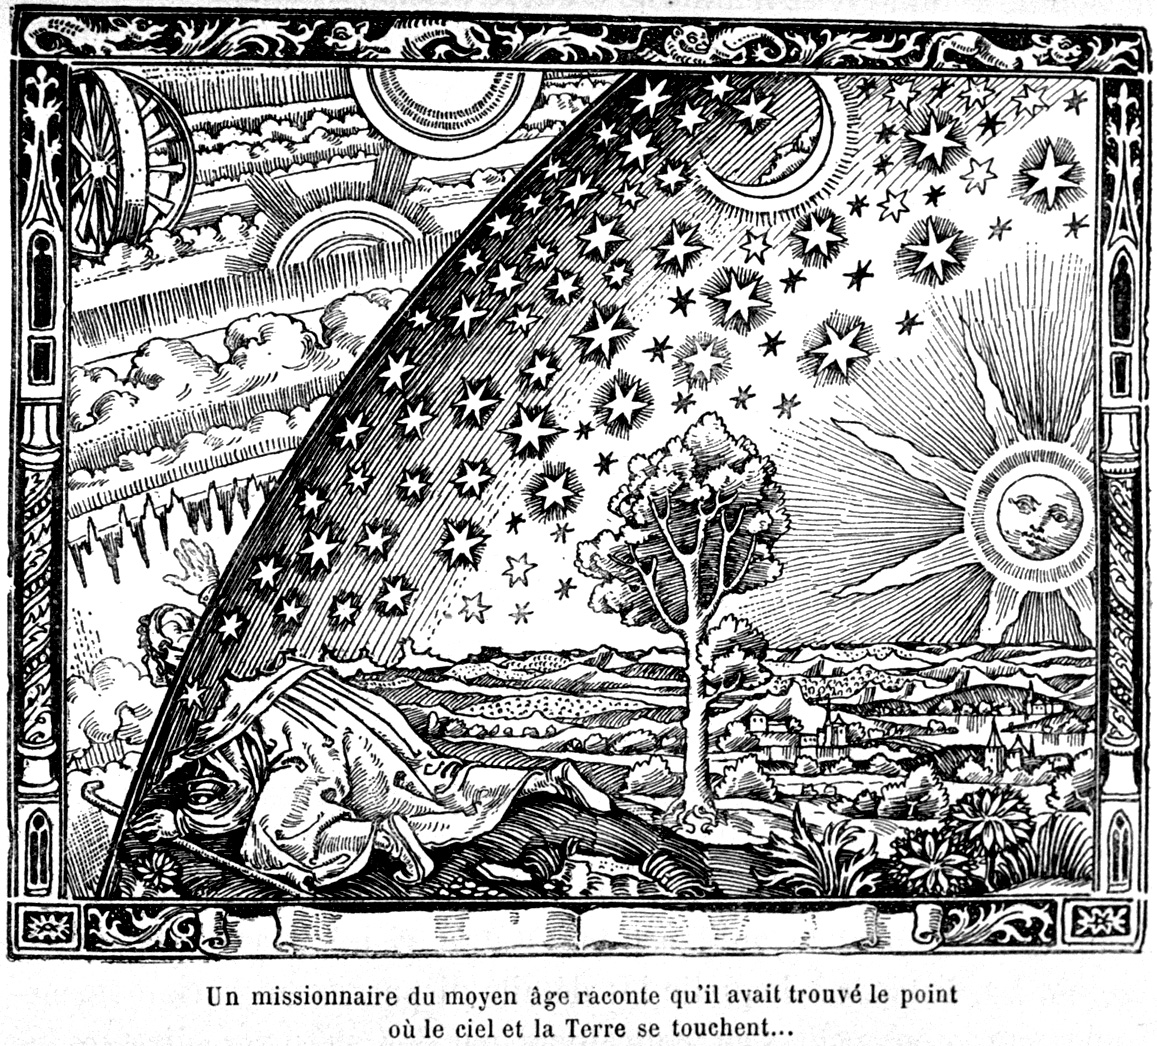
\includegraphics[scale=0.3]{img/Flammarion.eps}
 \captionsetup{labelformat=empty}
 \caption{1888年在巴黎出版的《弗拉马利翁》木刻版画,第163页,作者为无名氏}
 \label{fig:Flamarion-woodcut}
\end{figure}

%% Camille Flammarion, L'Atmosphere: Météorologie Populaire (Paris, 1888), p. 163.

%% The Flammarion Woodcut is an enigmatic woodcut by an unknown artist. It is referred to as the Flammarion Woodcut because its first documented appearance is in page 163 of Camille Flammarion's L'atmosphère: météorologie populaire (Paris, 1888), a work on meteorology for a general audience. The woodcut depicts a man peering through the Earth's atmosphere as if it were a curtain to look at the inner workings of the universe.

%% The original caption bellow the picture translated to: "A medieval missionary (Bruno) tells that he has found the point where heaven and Earth meet...".

1888年在巴黎出版的一幅木刻版画反映了当时人们对于有穷世界边沿的思考。一个人如果站在天球的边沿,是否可以伸出自己的手臂或者举起一根手杖?如果不可以,这显然是难以理解的,如果可以,那么处于物质世界外围的空间是什么?这就是宇宙边缘悖论。为了解决这个难题,中世纪的基督教重塑了亚里士多德的学说,提出了一种渐进边缘理论。还有人为,如果在宇宙的边缘向外抛出一支矛,就会推动宇宙扩大。物质世界是有界的,但界被无尽的虚空包围。

文艺复兴时期,数学逐渐被当时艺术大师们引入到作品中。达芬奇不仅深谙解刨和透视,还有意识地在在作品中使用引发美感的比例。这一时期的德国画家丢勒仔细研究了人体的各种比例,甚至利用坐标格点来描述透视的关系。丢勒的《量度四书》既介绍了绘画理论,也对几何原理和透视原理进行了研究。随后开普勒和笛沙格独立发展出了摄影几何中的无穷远点概念。笛沙格概括消失点的用途,纳入无穷远时的情形,发展出建构透视图的另一种方法。他让平行线确实平行的欧氏几何成为所有可能的几何系统都会有的特例。

\index{非欧几何}
真正从本质上改变了艺术家的视角,使得人们能够直接表现无穷要从非欧几何的诞生说起。长期以来,欧几里得几何被人们认为是完美的公理系统和演绎推理的典范。但是追求尽善尽美的数学家对于欧几里得第五公设颇有微词。前几条公设简单直观,符合直觉,例如说两点之间能够画一条直线,所有直角都相等。而第五公设描述却比较复杂。它说如果某条直线与两直线相交,且同侧两个内角和小于两个直角,那么两条直线无限延长后就会在该侧相交。第五公设也叫作平行公设,它等价于说,在平面内过直线外一点有且仅有一条平行线。人们感觉第五公设能从前面四条公设里推导出,并且实际上欧几里得在《几何原本》前面相当大的部分也都没有使用第五公设。在其后的两千多年里,很多人试图证明第五公设,但都失败了。于是意大利数学家撒凯里(Saccheri)尝试用反证法来证明,他假定第五公设不成立,然后导出一整套几何系统和奇怪的结论,接下来他宣称这些结果太过荒谬,从而说明第五公设是必定是正确的。

19世纪,德国数学家高斯、俄国数学家罗巴切夫斯基、匈牙利数学家波尔约等人各自独立地认识到这种证明是不可能的。也就是说,平行公理是独立于其他公理的,并且可以用不同的“平行公理”来替代它。高斯关于非欧几何的信件和笔记在他生前一直没有公开发表,只是在他1885年去世后出版时才引起人们的注意。罗巴切夫斯基和波尔约分别在1830年前后发表了他们关于非欧几何的理论。在这种几何里,罗巴切夫斯基平行公理替代了欧几里得平行公理,即在一个平面上,过已知直线外一点至少有两条直线与该直线不相交。由此可演绎出一系列全无矛盾的结论,并且可以得出三角形的内角和小于两直角。罗氏几何中有许多不同于欧氏几何的定理。

继罗氏几何后,德国数学家黎曼在1854年又提出了既不是欧氏几何也不是罗氏几何的新的非欧几何。这种几何采用如下公理替代欧几里得平行公理:同一平面上的任何两直线一定相交。同时,还对欧氏几何的其他公理做了部分改动。在这种几何里,三角形的内角和大于两直角。人们把这种几何称为椭圆几何。

直到1866年,意大利数学家贝尔特拉米在他出版的《非欧几何解释的尝试》中,证明了非欧平面几何可以局部地在欧氏空间中实现。1871年,德国数学家克莱因认识到从射影几何中可以推导度量几何,并建立了非欧几何模型。这样,非欧几何的相容性问题就归结为欧氏几何的相容性问题,由此非欧几何得到了普遍的承认。

%\begin{wrapfigure}{L}{0.4\textwidth}
\begin{figure}[htbp]
 \centering
 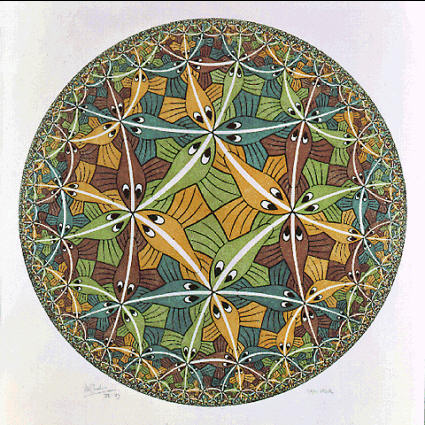
\includegraphics[scale=1.0]{img/circle-limit-III-1959.eps}
 \captionsetup{labelformat=empty}
 \caption{埃舍尔《圆极限$\cdot$3》1959}
 \label{fig:circle-limit-3}
\end{figure}
%\end{wrapfigure}

非欧几何向我们揭示这样一种可能性,即无穷的空间可能是有界的。法国数学家庞加莱在他的科普读物《科学与假设》中介绍了这样一种有趣的世界。整个世界被一个大小有限的球包围起来。中心的温度很高,随着远离中心,温度成比例地减小。当接近包围这这个世界的球面时,温度降到绝对零度。如果大球的半径是$R$,某点到球心的距离是$r$,则温度与$R^2 - r^2$成比例。这个世界中,由于热胀冷缩,物体的大小和温度成比例,越接近世界的边沿,物体越小。于是就出现这样的一个奇观,当这个世界的居民接近球面时,温度越来越低,他们越来越小,步伐也越来越小,他们永远也到不了世界的边沿,尽管这个世界是有限的。庞加莱描述的这个世界,实际上起作用的几何是一种称为双曲几何的非欧几里得几何学。

荷兰画家埃舍尔受到庞加莱的启发,创作了多个艺术作品来描述这种有限但无穷的世界。这一系列作品被命名为圆极限系列。不管是天使、魔鬼、还是游动的鱼,都在接近圆盘的边缘时变小,从而永远无法到达这个有界但无穷的边沿。

不仅是艺术,在音乐中也有对无穷的思索和表现。1747年5月,巴赫访问了波茨坦宫廷圣苏西宫。巴赫到了圣苏西宫后,腓特烈大帝向他展示了刚刚引进的吉尔博曼钢琴。宫廷音乐会上腓特烈大帝给了巴赫一个音乐主题,老巴赫当场即兴对其进行了一个三声部的赋格变奏。这是事前毫无演练的即兴演奏。这不仅使大帝十分满意,在场众人也无不瞠目结舌。巴赫本人觉得这首曲子的主题非常美丽,于是打算将来写成一首赋格曲,以供出版。回到莱比锡后,巴赫重新对国王主题进行变奏创作,将整个曲子按两首赋格曲,四乐章三重奏鸣曲和十首卡农的构成完成了整个曲子。巴赫在献词上所署名的时间正好是7月7日。这就是巴赫的经典名作《音乐的奉献》,乐曲编号BWV1079。在其中有一首极不寻常的卡农,只标着“Canon per Tonos”这三个词。翻译过来的意思是经由种种调性的卡农。后人称之为“无穷升高的卡农”。侯世达在《哥德尔、埃舍尔、巴赫——集异璧之大成》一书中写到:

\begin{figure}[htbp]
%\begin{wrapfigure}{R}{0.4\textwidth}
 \centering
 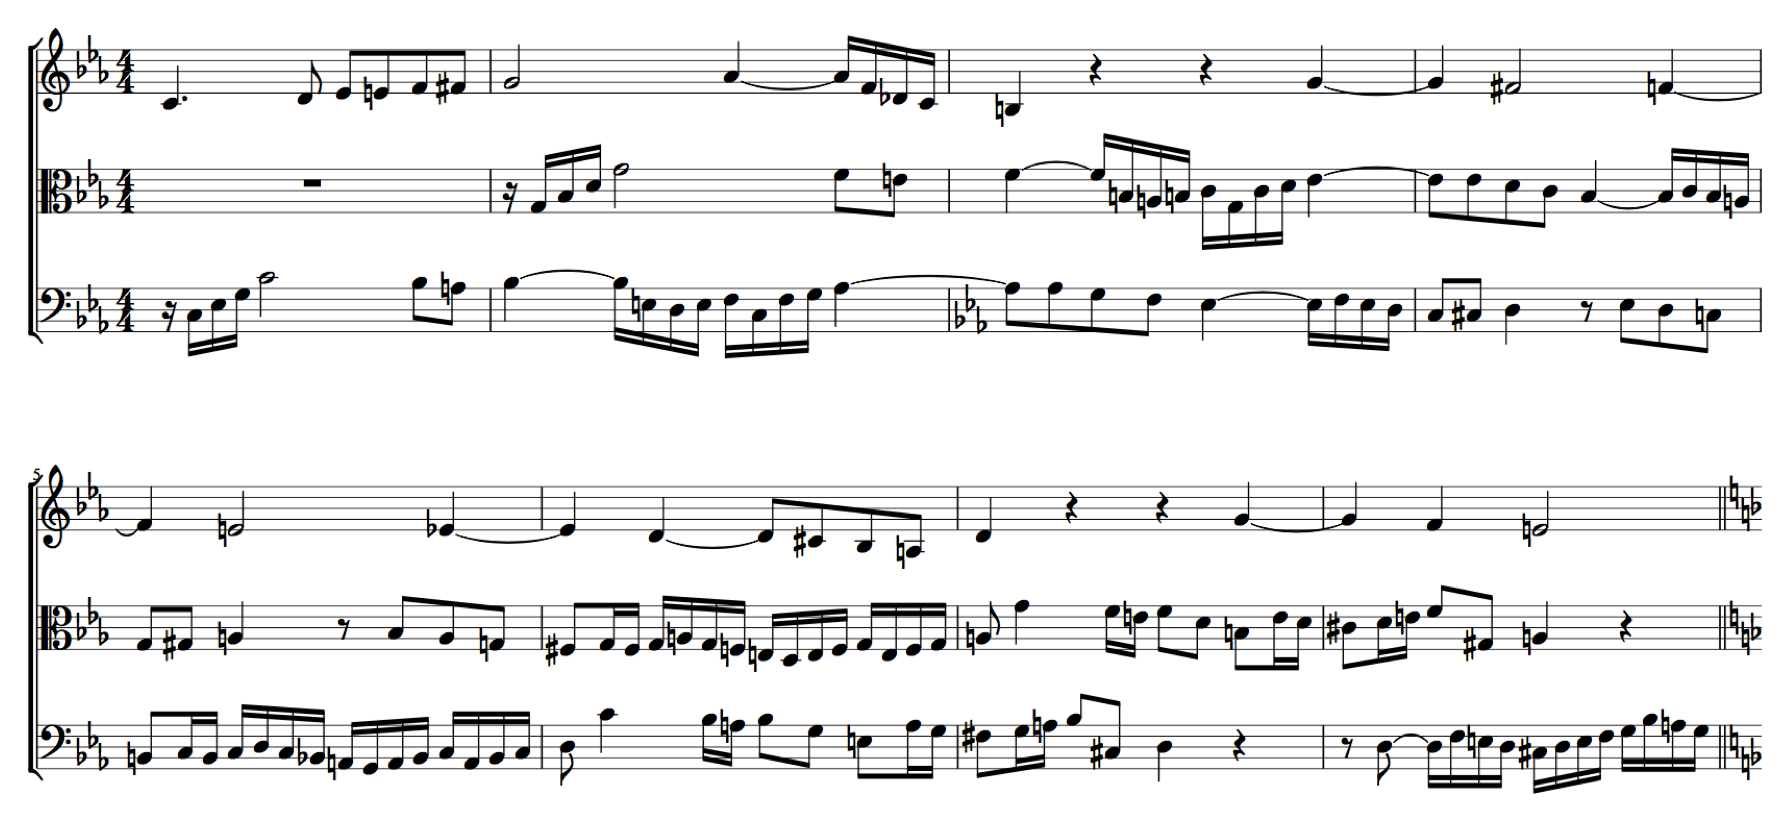
\includegraphics[scale=0.3]{img/canon-endless.eps}
 \captionsetup{labelformat=empty}
 \caption{巴赫创作的无穷升高的卡农的曲谱局部}
 \label{fig:canon-endless}
%\end{wrapfigure}
\end{figure}

它有三个声部,最高声部是国王主题的一个变奏,下面两个声部则提供了一个建立在第二主题之上的卡农化的和声。这两个声部中较低的那个声部用C小调奏出主题,而较高的那个则在差五度之上奏出同一主题。特殊之处在于,当它结束时——或者不如说似乎要结束时——已不再是C小调而是D小调了。巴赫在听众的鼻子底下转了调。而且这一结构使得这一“结尾”很通顺地与开头联接起来。这样可以重复这一过程并在E调上回到开头。这些连续的变调带着听众不断上升到越来越远的调区,因此听了几段之后,听众会以为他要无休止地远离开始的调子了。然而在整整六次这样的变调之后,原来的C小调又魔术般地恢复了!所有的声音都恰好比原来高八度。在这里整部曲子可以以符合音乐规则的方式终止。人们猜想,这里就是巴赫的意图。但巴赫很明确地留下了一个暗示,说这一过程可以无休止地进行下去。也许这就是为什么他在边上写下了“转调升高,国王的荣耀也升高。”\cite{GEB}

\begin{Exercise}
\Question{在两个镜子中间点燃一支蜡烛,你看到了什么?这是潜无穷还是实无穷?}
\end{Exercise}

\section{附录:例子代码}

使用流定义自然数潜无穷,并取出前15个自然数。Java语言1.8中的例子:

\lstset{frame=single, language=Java}
\begin{lstlisting}
IntStream.iterate(1, i -> i + 1);

IntStream.iterate(1, i -> i + 1)
        .limit(15).forEach(System.out::println);
\end{lstlisting}

Python语言版本3中的例子:

\lstset{frame=single, language=Python}
\begin{lstlisting}
def naturals():
    yield 0
    for n in naturals():
        yield n + 1
\end{lstlisting}

Haskell语言中使用递归定义自然数潜无穷:

\lstset{frame=single, language=Haskell}
\begin{lstlisting}
nat = 1 : (map (+1) nat)

take 15 nat
\end{lstlisting}

Haskell语言中使用递归定义斐波那契数列潜无穷,以及计算第1500个斐波那契数。

\lstset{frame=single, language=Haskell}
\begin{lstlisting}
fib = 0 : 1 : zipWith (+) fib (tail fib)

take 15 fib
[0,1,1,2,3,5,8,13,21,34,55,89,144,233,377]

fib !! 1500
13551125668563101951636936867148408377786010712418497242133543153221487310
87352875061225935403571726530037377881434732025769925708235655004534991410
29242495959974839822286992875272419318113250950996424476212422002092544399
20196960465321438498305345893378932585393381539093549479296194800838145996
187122583354898000
\end{lstlisting}

Haskell语言中使用余代数定义素数的潜无穷流

\lstset{frame=single, language=Haskell}
\begin{lstlisting}
data StreamF e a = StreamF e a
data Stream e = Stream e (Stream e)

takeStream 0 _ = []
takeStream n (Stream e s) = e : takeStream (n - 1) s

era (p:ns) = StreamF p (filter (p `notdiv`) ns)
  where notdiv p n = n `mod` p /= 0

primes = ana era [2..]

takeStream 15 primes
[2,3,5,7,11,13,17,19,23,29,31,37,41,43,47]
\end{lstlisting}

\section{附录:康托尔定理的证明}

\begin{theorem}
\textbf{康托尔定理}:对于任意集合都有$|S| < |2^S|$,其中$|S|$表示集合$S$的势,$2^S$表示$S$的幂集,即$S$的所有子集组成的集合。
\end{theorem}

\begin{proof}
我们分两步证明。首先证明$|S| \leq |2^S|$。对于任一$x$,令$f(x) = \{x\}$,也就是仅含有$x$唯一元素的集合。对于不同的元素$x_1 \neq x_2$,自然有$\{x_1\} \neq \{x_2\}$,即$f(x_1) \neq f(x_2)$。从而映射$S \arrowto{f} 2^S$是一单射。因此有
\[
  |S| \leq |2^S|
\]

第二步,我们证明$|S| \neq |2^S|$。采用反证法,假设等号成立。则存在一一映射$S \arrowto{\phi} 2^S$,使得对任一$x \in S$,都有$\phi(x) \in 2^S$。即$\phi(x)$是$S$的某个子集,所以$\phi(x) \subseteq S$。现在要问:$x$是否属于$\phi(x)$?有两种可能:一种是$x \in \phi(x)$,也可能是$x \notin \phi(x)$。我们把所有$x$不属于$\phi(x)$的元素放在一起构造一个新集合$S_0$:

\be
S_0 = \{ x | x \in S, \text{并且} x \notin \phi(x)\}
\label{eq:def-s0}
\ee

显然$S_0$是$S$的子集,即$S_0 \subseteq S$,因此$S_0 \in 2^S$。由于$\phi$是一一映射,所以必然存在一个$x_0$,使得$\phi(x_0) = S_0$。根据逻辑中的排中律,要么$x_0 \in S_0$,要么$x_0 \notin S_0$,二者必居其一,且仅有一个成立。

接下来分情况讨论。如果$x_0 \in S_0$成立,根据式(\ref{eq:def-s0})中$S_0$的定义,应该有$x_0 \notin \phi(x_0)$,由于$\phi(x_0) = S_0$,所以$x_0 \notin S_0$。

如果$x_0 \notin S_0$,因为$S_0 = \phi(x_0)$,所以得到$x_0 \notin \phi(x_0)$。这样根据$S_0$的定义(\ref{eq:def-s0}),又应该有$x_0 \in S_0$。

这样不论$x_0$是否属于$S_0$,都导致矛盾。这说明我们最初的假设$S$到$2^S$间存在一一映射是错误的。所以不等式$|S| \neq |2^S|$成立。

由这两步的结果:$|S| \leq |2^S|$,并且$|S| \neq |2^S|$,我们得到了康托尔定理的结论:

\[
  |S| < |2^S|
\]
\end{proof}

证明的第二部分,不由让我们联想起了著名的罗素悖论:令$S$为所有不属于自己的集合构成的集合,问$S$是否属于自己?我们将在下一章讲述罗素悖论和哥德尔不完全性定理。

% Mathematicians aren't satisfied because they know there are no solutions up to four million or four billion, they really want to know that there are no solutions up to infinity. -- Andrew Wiles

\section{附录:巴赫《音乐的奉献》无限上升的卡农}

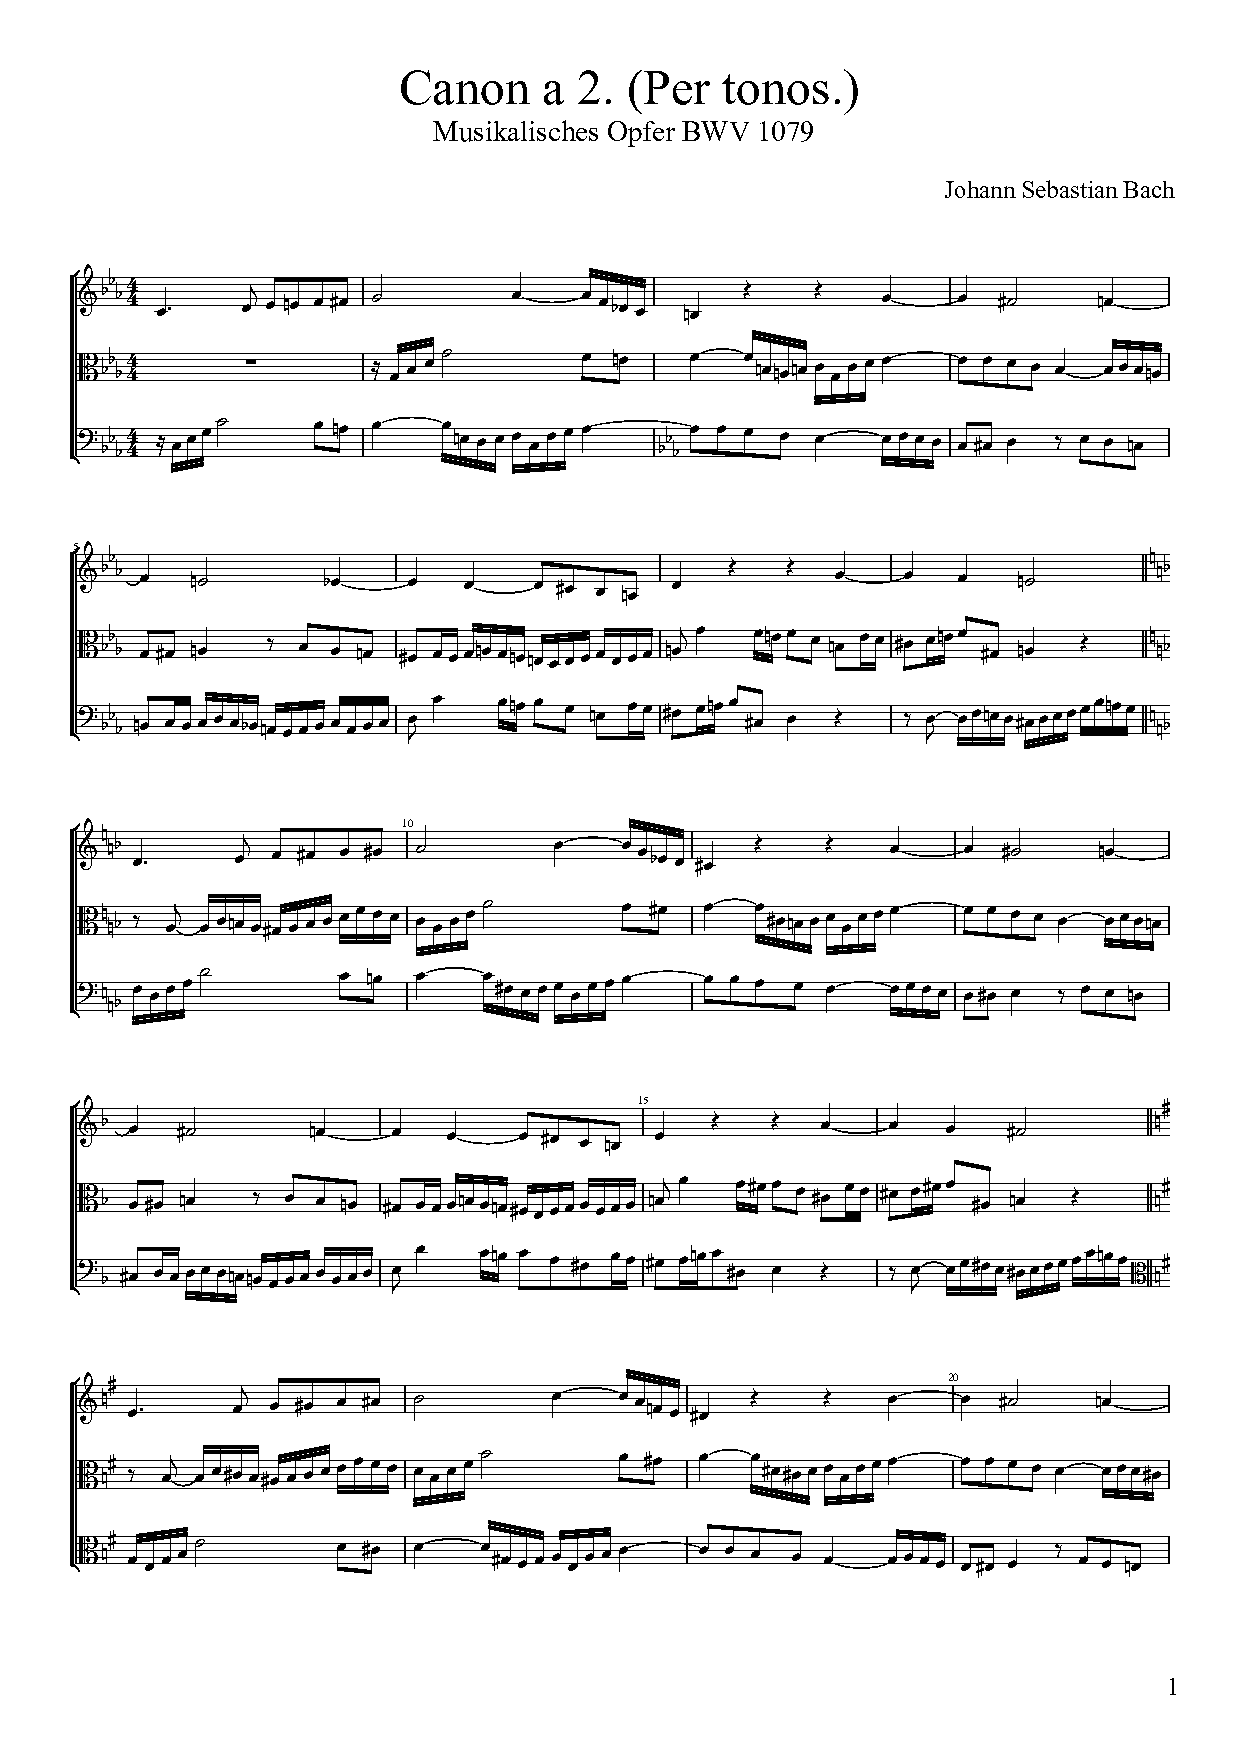
\includepdf[pages=-,
nup=2x2
, scale=0.85
%,fitpaper=true
]{img/bwv1079-canon-per-tonos.pdf}

\ifx\wholebook\relax \else
\begin{thebibliography}{99}

\bibitem{De-linfini-2018}
[法] 让-皮埃尔$\cdot$卢米涅,马克$\cdot$拉雪茨-雷 著,孙展 译. 从无穷开始——科学的困惑与疆界. 人民邮电出版社. 2018. ISBN: 9787115479198

\bibitem{Noguchi2007}
[日] 野口哲也 著,刘慧 韩丽红 译. 数学原来可以这样学. 湖南人民出版社. 2014. ISBN: 9787556100897
% Tetsunori Noguchi. SUGAKUTEKI SENSE GA MINITUKU RENSHUCHO.

\bibitem{Wikipedia-Googol}
Wikipedia. ``Googol''. \url{https://en.wikipedia.org/wiki/Googol}

\bibitem{Wikipedia-Zeno}
Wikipedia. ``Zeno's Paradoxes''. \url{https://en.wikipedia.org/wiki/Zeno's_paradoxes}

\bibitem{HanXueTao16}
韩雪涛 ``数学悖论与三次数学危机''. 人民邮电出版社. 2016, ISBN: 9787115430434

\bibitem{Elements}
[古希腊] 欧几里得 著,兰纪正 朱恩宽 译,梁宗巨 张毓新 徐伯谦 校订 ``几何原本''. 译林出版社. 2014, ISBN: 9787544750066

\bibitem{M-Kline-2007}
[美] M$\cdot$克莱因 著 李宏魁 译 ``数学:确定性的丧失'' 湖南科学技术出版社,2007年4月 ISBN: 978-7-5357-1857-0
% Morris Kline ``Mathematics: The Loss of Certainty''. Oxford University Press, 1980.

\bibitem{Stepanov}
Stepanov and Rose. ``数学与泛型编程''. 爱飞翔译,机械工业出版社。ISBN: 978-7-111-57658-7. 2017.

\bibitem{GEB}
[美]候世达 ``哥德尔、埃舍尔、巴赫——集异壁之大成''. 商务印书馆 1996. ISBN: 978-7-100-01323-9

\bibitem{GCH}
张锦文,王雪生 ``连续统假设''. 世界数学名题欣赏丛书。辽宁教育出版社 1988. ISBN: 7-5382-0436-9/G$\cdot$445

\bibitem{Courant1969}
[美] R$\cdot$柯朗, H$\cdot$罗宾 著,[英] I$\cdot$斯图尔特 修订,左平,张饴慈 译 ``什么是数学:对思想和方法的基本研究(中文版第四版)''. 上海:复旦大学出版社 2017,ISBN: 9787309086232.

% Richard Courant, Herbert Robbins , Reviewed by Ian Stewart. ``What Is Mathematics? An Elementary Approach to Ideas and Methods 2nd Edition''. Oxford University Press,  1996, ISBN: 978-0195105193.

\bibitem{Poincare1}
[法]彭加勒 著,李醒民 译 ``科学与假设'' 商务印书馆. 2006. ISBN: 978-7-100-04796-8

\end{thebibliography}

\expandafter\enddocument
%\end{document}

\fi
